%%% The main file. It contains definitions of basic parameters and includes all other parts.

%% Settings for single-side (simplex) printing
% Margins: left 40mm, right 25mm, top and bottom 25mm
% (but beware, LaTeX adds 1in implicitly)
\documentclass[12pt,a4paper]{report}
\setlength\textwidth{145mm}
\setlength\textheight{247mm}
\setlength\oddsidemargin{15mm}
\setlength\evensidemargin{15mm}
\setlength\topmargin{0mm}
\setlength\headsep{0mm}
\setlength\headheight{0mm}
% \openright makes the following text appear on a right-hand page
\let\openright=\clearpage

%% Settings for two-sided (duplex) printing
% \documentclass[12pt,a4paper,twoside,openright]{report}
% \setlength\textwidth{145mm}
% \setlength\textheight{247mm}
% \setlength\oddsidemargin{14.2mm}
% \setlength\evensidemargin{0mm}
% \setlength\topmargin{0mm}
% \setlength\headsep{0mm}
% \setlength\headheight{0mm}
% \let\openright=\cleardoublepage


% All packages are imported here

%% Generate PDF/A-2u
\usepackage[a-2u]{pdfx}

%% Character encoding: usually latin2, cp1250 or utf8:
\usepackage[utf8]{inputenc}

%% Prefer Latin Modern fonts
\usepackage{lmodern}

%% Further useful packages (included in most LaTeX distributions)
\usepackage{amsmath}        % extensions for typesetting of math
\usepackage{amsfonts}       % math fonts
\usepackage{amsthm}         % theorems, definitions, etc.
\usepackage{bbding}         % various symbols (squares, asterisks, scissors, ...)
\usepackage{bm}             % boldface symbols (\bm)
\usepackage{graphicx}       % embedding of pictures
\usepackage{fancyvrb}       % improved verbatim environment
%\usepackage{natbib}         % citation style AUTHOR (YEAR), or AUTHOR [NUMBER]
\usepackage[nottoc]{tocbibind} % makes sure that bibliography and the lists
			    % of figures/tables are included in the table
			    % of contents
\usepackage{dcolumn}        % improved alignment of table columns
\usepackage{booktabs}       % improved horizontal lines in tables
\usepackage{paralist}       % improved enumerate and itemize
\usepackage{xcolor}         % typesetting in color

\usepackage[toc,acronym]{glossaries}
%%% Basic information on the thesis

% Thesis title in English (exactly as in the formal assignment)
\def\ThesisTitle{GPU Parallelization of Evolutionary Algorithms}

% Author of the thesis
\def\ThesisAuthor{Patrik Valkovič}

% Year when the thesis is submitted
\def\YearSubmitted{2021}

% Name of the department or institute, where the work was officially assigned
% (according to the Organizational Structure of MFF UK in English,
% or a full name of a department outside MFF)
\def\Department{Department of Theoretical Computer Science and Mathematical Logic}

% Is it a department (katedra), or an institute (ústav)?
\def\DeptType{Department}

% Thesis supervisor: name, surname and titles
\def\Supervisor{Mgr. Martin Pilát, Ph.D.}

% Supervisor's department (again according to Organizational structure of MFF)
\def\SupervisorsDepartment{Department of Theoretical Computer Science and Mathematical Logic}

% Study programme and specialization
\def\StudyProgramme{Computer Science}
\def\StudyBranch{Artificial Intelligence}

% Abstract (recommended length around 80-200 words; this is not a copy of your thesis assignment!)
\def\Abstract{%
\acrlongpl*{acc:gpu} stand for the success of \acrlong*{acc:ai} over the last decade and their broader application in the industry. Another promising field of \acrlong*{acc:ai} is \acrlong*{acc:ea}. Their parallelization ability is well known and has been successfully applied in practice. However, these attempts focused on multi--core and multi--machine parallelization rather than on the \acrshort*{acc:gpu}.\\
This work explores the possibilities of \acrlong*{acc:ea} parallelization on \acrshort*{acc:gpu}. I propose implementation in PyTorch library, allowing execution of \acrshort*{acc:ea} on \acrshort*{acc:gpu}. The proposed implementation provides the most common evolutionary operators for \acrlongpl*{acc:ga}, Real--Coded Evolutionary Algorithms, and \acrlong*{acc:pso} Algorithms. Finally, I show the performance is by order of magnitude faster on \acrshort*{acc:gpu} for medium and big--sized problems and populations.
}

% 3 to 5 keywords (recommended), each enclosed in curly braces
\def\Keywords{%
{Evolutionary Algorithms}, {Parallelization}, {GPU Computing}, {Genetic Algorithms}, {Particle Swarm Optimization}
}
% An optional dedication: you can thank whomever you wish (your supervisor,
% consultant, a person who lent the software, etc.)
\def\Dedication{%
I wish to thank my supervisor, Mgr. Martin Pilát, Ph.D., for his guidance, help, and mostly patience during my work on this thesis. I am thankful for his friendly attitude and valuable advice.

I would also want to express my sincere gratitude to my family and friends, without which support this work would not have been possible.

Computational resources were supplied by the project "e-Infrastruktura CZ" (e-INFRA LM2018140) provided within the program Projects of Large Research, Development and Innovations Infrastructures.
I would like to thank Cesnet for allowing me to use the computational power of MetaCentrum for the purpose of this thesis. I could not get presented results without their support.
}
%%% This file contains definitions of various useful macros and environments %%%
%%% Please add more macros here instead of cluttering other files with them. %%%

%%% Minor tweaks of style

% These macros employ a little dirty trick to convince LaTeX to typeset
% chapter headings sanely, without lots of empty space above them.
% Feel free to ignore.
\makeatletter
\def\@makechapterhead#1{
  {\parindent \z@ \raggedright \normalfont
   \Huge\bfseries \thechapter. #1
   \par\nobreak
   \vskip 20\p@
}}
\def\@makeschapterhead#1{
  {\parindent \z@ \raggedright \normalfont
   \Huge\bfseries #1
   \par\nobreak
   \vskip 20\p@
}}
\makeatother

% This macro defines a chapter, which is not numbered, but is included
% in the table of contents.
\def\chapwithtoc#1{
\chapter*{#1}
\addcontentsline{toc}{chapter}{#1}
}

% Draw black "slugs" whenever a line overflows, so that we can spot it easily.
\overfullrule=1mm

%%% Macros for definitions, theorems, claims, examples, ... (requires amsthm package)

\theoremstyle{plain}
\newtheorem{thm}{Theorem}
\newtheorem{lemma}[thm]{Lemma}
\newtheorem{claim}[thm]{Claim}

\theoremstyle{plain}
\newtheorem{defn}{Definition}

\theoremstyle{remark}
\newtheorem*{cor}{Corollary}
\newtheorem*{rem}{Remark}
\newtheorem*{example}{Example}

%%% An environment for proofs

\newenvironment{myproof}{
  \par\medskip\noindent
  \textit{Proof}.
}{
\newline
\rightline{$\qedsymbol$}
}

%%% An environment for typesetting of program code and input/output
%%% of programs. (Requires the fancyvrb package -- fancy verbatim.)

\DefineVerbatimEnvironment{code}{Verbatim}{fontsize=\small, frame=single}

%%% The field of all real and natural numbers
\newcommand{\R}{\mathbb{R}}
\newcommand{\N}{\mathbb{N}}

%%% Useful operators for statistics and probability
\DeclareMathOperator{\pr}{\textsf{P}}
\DeclareMathOperator{\E}{\textsf{E}\,}
\DeclareMathOperator{\var}{\textrm{var}}
\DeclareMathOperator{\sd}{\textrm{sd}}

%%% Transposition of a vector/matrix
\newcommand{\T}[1]{#1^\top}

%%% Various math goodies
\newcommand{\goto}{\rightarrow}
\newcommand{\gotop}{\stackrel{P}{\longrightarrow}}
\newcommand{\maon}[1]{o(n^{#1})}
\newcommand{\abs}[1]{\left|{#1}\right|}
\newcommand{\dint}{\int_0^\tau\!\!\int_0^\tau}
\newcommand{\isqr}[1]{\frac{1}{\sqrt{#1}}}

%%% Various table goodies
\newcommand{\pulrad}[1]{\raisebox{1.5ex}[0pt]{#1}}
\newcommand{\mc}[1]{\multicolumn{1}{c}{#1}}

\newcommand{\defterm}[1]{\vspace{0.6em}\noindent\textbf{#1}}

\newcommand{\individual}{\pmb{p}}
\newcommand{\population}{\mathcal{P}}
\newcommand{\fitnessfn}{f_f}
\newcommand{\objectivefn}{f_o}

\DeclareMathOperator*{\argmax}{arg\,max}
\DeclareMathOperator*{\argmin}{arg\,min}
\newcommand{\norm}[1]{\left\lVert#1\right\rVert}

\newcommand{\snipescondition}{increase variety of the population}
\makeglossaries

\newacronym{acc:ann}{ANN}{Artificial Neural Networks}
\newacronym{acc:ai}{AI}{Artificial intelligence}
\newacronym{acc:dann}{DANN}{Deep Artificial Neural Networks}
\newacronym{acc:cnn}{CNN}{Convolutional Neural Networks}
\newacronym[plural=GPUs,firstplural=Graphical Processing Units (GPUs)]{acc:gpu}{GPU}{Graphical Processing Unit}
\newacronym{acc:tpu}{TPU}{Tensor Processing Unit}
\newacronym{acc:cuda}{CUDA}{Compute Unified Device Architecture}
\newacronym[plural=EAs]{acc:ea}{EA}{Evolutionary Algorithms}
\newacronym[plural=GAs, firstplural=Genetic Algorithms]{acc:ga}{GA}{Genetic Algorithm}
\newacronym{acc:es}{ES}{Evolution Strategies}
\newacronym{acc:pso}{PSO}{Particle Swarm Optimization}
\newacronym{acc:dna}{DNA}{Deoxyribonucleic Acid}
\newacronym{acc:tsp}{TSP}{Traveling Salesman Problem}
\newacronym{acc:blx}{BLX}{Blend Crossover}
\newacronym{acc:cma}{CMA--ES}{Covariance Matrix Adaptation -- Evolution Strategy}
\newacronym{acc:de}{DE}{Differential evolution}
\newacronym{acc:spso2006}{SPSO--2006}{Standard Particle Swarm Optimization 2006}  
\newacronym{acc:spso2011}{SPSO--2011}{Standard Particle Swarm Optimization 2011}  
\newacronym[plural=CPUs,firstplural=Central Processing Units (CPUs)]{acc:cpu}{CPU}{Central Processing Unit}
\newacronym{acc:ghz}{GHz}{gigahertz}
\newacronym{acc:mhz}{MHz}{megahertz}
\newacronym[plural=APIs,firstplural=Application Programming Interfaces (APIs)]{acc:api}{API}{Application Programming Interface}
\newacronym[plural=SMs, firstplural=Stream Multiprocessors]{acc:sm}{SM}{Stream Multiprocessor}
\newacronym[plural=SPs, firstplural=Stream Processors]{acc:sp}{SP}{Stream Processor}
\newacronym{acc:simd}{SIMD}{Single Instruction, Multiple Data}
\newacronym{acc:os}{OS}{Operating System}
\newacronym{acc:bbob}{BBOB}{Black--Box Optimization Benchmarking}
\newacronym{acc:coco}{COCO}{Comparing Continuous Optimizers}
\newacronym{acc:ffeat}{FFEAT}{Framework For Evolution Algorithms in Torch}
\newacronym{acc:sus}{SUS}{Stochastic Universal Sampling}
\newacronym{acc:sat}{SAT}{Boolean Satisfiability Problem}
\newacronym{acc:3sat}{3SAT}{\acrshort{acc:sat} problems with exactly three literals in clause}

%% The hyperref package for clickable links in PDF and also for storing
%% metadata to PDF (including the table of contents).
%% Most settings are pre-set by the pdfx package.
\hypersetup{unicode}
\hypersetup{breaklinks=true}

% Title page and various mandatory informational pages
\begin{document}
%%% Title page of the thesis and other mandatory pages

%%% Title page of the thesis

\pagestyle{empty}
\hypersetup{pageanchor=false}
\begin{center}

\centerline{\mbox{
\includegraphics[width=166mm]{img/logo-en.pdf}}}

\vspace{-8mm}
\vfill

{\bf\Large MASTER THESIS}

\vfill

{\LARGE\ThesisAuthor}

\vspace{15mm}

{\LARGE\bfseries\ThesisTitle}

\vfill

\Department

\vfill

{
\centerline{\vbox{\halign{\hbox to 0.45\hsize{\hfil #}&\hskip 0.5em\parbox[t]{0.45\hsize}{\raggedright #}\cr
Supervisor of the master thesis:&\Supervisor \cr
\noalign{\vspace{2mm}}
Study programme:&\StudyProgramme \cr
\noalign{\vspace{2mm}}
Study branch:&\StudyBranch \cr
}}}}

\vfill

% Zde doplňte rok
Prague \YearSubmitted

\end{center}

\newpage

%%% Here should be a bound sheet included -- a signed copy of the "master
%%% thesis assignment". This assignment is NOT a part of the electronic
%%% version of the thesis. DO NOT SCAN.

%%% A page with a solemn declaration to the master thesis

\openright
\hypersetup{pageanchor=true}
\pagestyle{plain}
\pagenumbering{roman}
\vglue 0pt plus 1fill

\noindent
I declare that I carried out this master thesis independently, and only with the cited
sources, literature and other professional sources. It has not been used to obtain another
or the same degree.

\medskip\noindent
I understand that my work relates to the rights and obligations under the Act No.~121/2000 Sb.,
the Copyright Act, as amended, in particular the fact that the Charles
University has the right to conclude a license agreement on the use of this
work as a school work pursuant to Section 60 subsection 1 of the Copyright~Act.

\vspace{10mm}

\hbox{\hbox to 0.5\hsize{%
In \hbox to 6em{\dotfill} date \hbox to 6em{\dotfill}
\hss}\hbox to 0.5\hsize{\dotfill\quad}}
\smallskip
\hbox{\hbox to 0.5\hsize{}\hbox to 0.5\hsize{\hfil Author's signature\hfil}}

\vspace{20mm}
\newpage

%%% Dedication

\openright

\noindent
\Dedication

\newpage

%%% Mandatory information page of the thesis

\openright

\vbox to 0.5\vsize{
\setlength\parindent{0mm}
\setlength\parskip{5mm}

Title:
\ThesisTitle

Author:
\ThesisAuthor

\DeptType:
\Department

Supervisor:
\Supervisor, \SupervisorsDepartment

Abstract:
\Abstract

Keywords:
\Keywords

\vss}

\newpage

\openright
\pagestyle{plain}
\pagenumbering{arabic}
\setcounter{page}{1}


%%% A page with automatically generated table of contents of the master thesis
\setcounter{tocdepth}{1}
\tableofcontents
% TODO fix document outline to generate subsection and table of content as well
% TODO right align proper pages

%%% Each chapter is kept in a separate file
\chapter{Introduction}

\acrfull{acc:ai} 
has become phenomenon of these days. Latest advances in this field achieved magnificent results and allowed creation of systems and tools, we though would be possible thirty years back. The biggest credit goes to the \acrfull{acc:ann}
, which allowed this rapid and astonishing growth of the field. More precisely, the \acrfull{acc:daan} 
sparkled this process in 2011, when they started to exceed human performance in German traffic sign recognition benchmark \cite{CIRESAN2012333}.
\chapter{\texorpdfstring{\acrlong*{acc:ea}}{}}

Optimization. What better word would describe the ultimate goal of all the people, our civilization, and maybe even the Universe. With a bit of exaggeration, optimization is the cause of all the ramifications we can see around. Because what else are Physic laws than minimization processes, our pursuit of knowledge and self improvement than maximization of self-worth, industrial revolutions than minimization of human labour, maximization of goods production and standard of living at the same time. In my opinion, optimization is the reason what drives us forward, makes us better, and guides our decisions.

One of the most extraordinary optimization processes is, without a doubt, evolution. Evolution is nothing less than Nature way of improvement species to better adapt to their environment. The father of evolution is undoubtedly Charles, who the first come up with an idea of evolution in his work \enquote{On the origin of species: A facsimile of the first edition} \citep{darwin1964origin}. According the him, the individuals that better adapted to the environment have higher potential to reproduce and pass their genetic material --- including the predisposition to survive in the environment --- to their offsprings. Sometimes referred as \enquote{Survival of the fittest}.

This exact ideas inspired scientists and formed the field of \acrfull{acc:ea}\index{evolutionary algorithm}\footnote{I will refer to all the population-based algorithms in this work as \acrlong*{acc:ea}. These includes, among others, \acrlong*{acc:ga}, \acrlong*{acc:ea}, and \acrlong*{acc:pso}.}.
\acrshort{acc:ea} are stochastic, population-based optimization algorithms inspired by biological evolution. In general, a set of individuals called population compete with each other for a place in the next generation. Each individual represent one possible solution of the problem in hand. Quality of the individual is proportional to the quality of solution it represents. This quality is usually expressed using fitness (or sometimes called objective) function. As with natural evolution, the probability of survival is proportional the solution quality -- the better the solution is, the higher the probability of survival \citep{IntroductionToEA}. In the \acrshort{acc:ea}, the process of producing new generation is usually called selection.

Evolution is not only about survival, but also about reproduction. \acrlong*{acc:ea} took inspiration here as well and uses specials operators for each generation -- usually called evolution operators or variation operators\index{variation operator}. As the name suggests, these operators make sure the population explores new solutions. The two most common operators are crossover and mutation. During crossover\index{crossover}, individuals from the current population (usually called parents) produces new individuals (usually called offsprings) by combining their genetic information. In some way, crossover mimic reproduction in Nature, during which the \acrshort{acc:dna} of offspring is by majority determined by its parents \acrshort{acc:dna}. Mutation\index{mutation}, on the other hand, causes random small alteration of the individual genetic material and is able to introduce novel patterns that did not previously occur in the population \citep{HowToSolveItModernHeuristics}.

In general, \acrshort{acc:ea} repeat steps above until sufficiently good solution is found, or until maximum number of generations is reached. The general pseudocode of the \acrshort{acc:ea} algorithm is in Algorithm \ref{alg:SEA}. I will present more accurate implementations of various algorithms thorough this chapter.

\begin{algorithm}
    \SetAlgoLined
    \KwResult{evolved population}
    initialize population\;
    \Repeat{termination criteria met}{
        reproduction\;
        mutation\;
        evaluate population\;
        selection\;
    }
    \caption{General Evolution Algorithm}
    \label{alg:SEA}
\end{algorithm}


%%%%%%%%%%%%%%%%%%%
%%               %%
%%  TERMINOLOGY  %%
%%               %%
%%%%%%%%%%%%%%%%%%%
\section{Terminology}

In this section, I will introduce necessary terminology that I am going to use thorough this work. I took most of the terminology from \citet{IntroductionToEA}.

\defterm{Problem} is the function we want to solve. It can be both satisfactory as well optimization problem.

\defterm{Genotype}\index{genotype} is encoding of the solution. It is equivalent of the \acrshort{acc:dna} -- it compress all the data needed to produce solution.

\defterm{Gene} is one part of the genotype. It may be one bit if the genotype is encoded as binary string or scalar, if the genotype is vector. 

\defterm{Representation or genotype space} is the space of genotype.

\defterm{Phenotype}\index{phenotype} is the solution built from genotype. Genotype and phenotype can be equivalent -- for example real function optimization problem may have as a genotype vector of real numbers, that represent one of the solution. Generally, however, genotype and phenotype can be different.

\defterm{Search space} is the space of phenotype.

\defterm{Objective function} is the function the algorithm optimize. For previous example of real function optimization, the function itself can be the objective function. I will denote objective function $\objectivefn$.

\defterm{Fitness function}\index{fitness function} is the measure of quality of the solution. Note that the domain of the function is the search space. Unlike the objective function, the fitness function should guide the algorithm during the optimization. It can use the objective function directly, but other options are possible as well. For example, if the goal is to maximize objective function $\objectivefn(x)$, but the algorithm is written such that it minimize the fitness function, one may specify the fitness function as $\fitnessfn(x)=\frac{1}{\objectivefn(x)}$. I will denote fitness function $\fitnessfn$.

\defterm{Evaluation} is the process of obtaining fitness value for the genotype.

\defterm{Individual} is genotype with it's fitness value. I will denote individual by $\individual$.

\defterm{Fitness value} of individual is it's evaluation. 

\defterm{Population} is multiset of individuals -- it is possible to have same genotype in the population multiple time. However, I will still distinguish different individuals with the same genotype. I will denote the whole population as $\population$.

\defterm{Initialization} is the process of creating the first population.

\defterm{Exploitation} is the effort to use knowledge from the history in order to maximize the expected outcome \citep{SelfAdaptiveFeaturesInRealParameterEvolutionaryAlgorithms}.

\defterm{Exploration} is the effort to discover new rules about the problem in hand, although the expected outcome does not need to be the best possible. In general, the biggest problem in \acrshort{acc:ea} is the right balance between exploitation and exploration. Putting too much emphasis may cause to get stuck in the local minima, whereas putting too much focus on the exploration may cause, that the algorithm never converge. Note that \acrshort{acc:ea} is not the only field suffering from this, but for example Reinforcement Learning deals with the same problems \citep{ExplorationExploitationDilemaRL}. 

\defterm{Evolution operators} are individual steps performed each iteration.

\defterm{Selection}\index{selection} is evolution operator that picks up individuals from the current population to the next one. The selection should take into account fitness of each individual in the population and pick them proportionally. Selection therefore implements the \enquote{Survival of the fittest} law. From the mathematical point of view, selection task is to move the population into more promising area of the search space and possibly to reduce variance of the population \citep{SelfAdaptiveFeaturesInRealParameterEvolutionaryAlgorithms}. In other word, selection is exploitation step in the algorithm.

\defterm{Crossover}\index{crossover} is evolution operator, that combines some individuals (usually called \textbf{parents}) in order to create one or more new individuals (usually called \textbf{offsprings}). Offsprings are usually combination of their parents, similarly to how \acrshort{acc:dna} of the child is combination of \acrshort{acc:dna} of her parents.

\defterm{Mutation}\index{mutation} is evolution operator, that modify one individual. Mutation can be based on randomness (for example replacement of value in genotype by different value) or specialized for the problem in hand. This time the example can be \acrlong{acc:tsp}, where one possible mutation operator can \enquote{untwist} ways that cross each other. This mutation is in fact local optimization technique, as the  mutated way is shorter than the previous one \citep{TSPArticle}.

\defterm{Variation operators}\index{variation operator} are operators, that change the variation of the population, but not the mean. Variation operators are the exploration steps in the algorithm and should balance the exploitation strength of the selection. Both crossover and mutation are variation operators \citep{SelfAdaptiveFeaturesInRealParameterEvolutionaryAlgorithms}.

\defterm{Memetic operator} is operator, that uses local optimization in every iteration. Alternatively, \enquote{memetic algorithms uses local optimizer to every solution before evaluation}\citep{HowToSolveItModernHeuristics}. One of such example is the \acrlong{acc:tsp} problem mentioned earlier. Another example is the problem of searching for weights in \acrshort{acc:ann}, where one step of backpropagation algorithm is performed as part of the mutation.




%%%%%%%%%%%%%%%%%%%%%%%%%%
%%                      %%
%%  GENETIC ALGORITHMS  %%
%%                      %%
%%%%%%%%%%%%%%%%%%%%%%%%%%
\section{\texorpdfstring{\acrlong*{acc:ga}}{}}

\acrfull{acc:ga} are probably the simplest \acrfull{acc:ea} out there and as their father is usually considered \citefullauthor{HollandGA}. In the \acrshort{acc:ga}, individual are binary string of length $n$, formally
$$ \individual \in \left\{0,1\right\}^{n} $$

Fitness function maps genotype into real values
$$ \fitnessfn:\left\{0,1\right\}^{n}\rightarrow\mathbb{R} $$

The typical crossover operator is one point crossover\index{crossover!one--point}. This type of crossover require two parents and produces two offsprings. As the first step, the algorithm uniformly sample random integer $s$ in the range $\left[ 1, n-1 \right]$. The first offspring will receive genetic material up to index $s$ from the first parent, and the rest from the second one. The second offspring is created the same way, except the position of parents is exchanged. Example for $n=10$ is in figure \ref{fig:gaonepointcrossover}. In order not to modify all the individuals in the population, only $p_c\in\left[0,1\right]$ percent of individuals undergo the crossover and the children replace their parents\citep{IntroductionToEA}.

\begin{figure}
    \begin{subfigure}[b]{0.4\textwidth}
        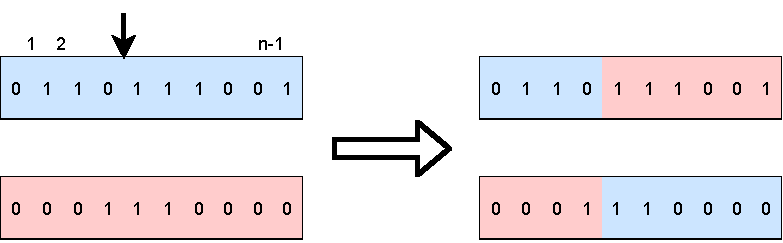
\includegraphics[width=\textwidth]{img/master_onepointcrossover.pdf}
        \caption{One point crossover}
        \label{fig:gaonepointcrossover}
    \end{subfigure}
    \hfill
    \begin{subfigure}[b]{0.4\textwidth}
        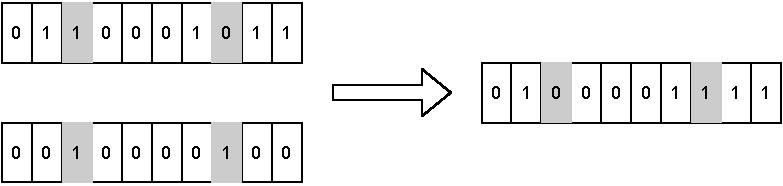
\includegraphics[width=\textwidth]{img/master_bitflipmutation.pdf}
        \caption{Bit-flip mutation}
        \label{fig:bitflipmutation}
    \end{subfigure}
    \caption{Genetic algorithm operators}
\end{figure}

The mutation\index{mutation} operator for \acrshort{acc:ga} is in most cases bit-flip mutation\index{mutation!bit-flip}. During this mutation, each gene in the genotype is mutated with probability $p_m$. One example of mutation is in figure \ref{fig:bitflipmutation}. Mutation has two objectives -- it makes sure the algorithm is not trapped in local optima, and it sustains genetic disparity in the population. As a side effect, mutation serves as minor search operator\citep{IntroToGA}.

The difference between crossover and mutation is such that crossover is rather \enquote{search} exploitation technique. It combines individuals from current population and exploit them to find possibly better individuals. Mutation, on the other hand, is more local search technique and based on the probability $p_b$ it search over the whole representation space.

Finally, the selection stage takes place. There are various selection techniques and in this particular case, I will use tournament selection\index{selection!tournament}. During tournament selection, fitness values of two random individuals are compared and the better individual is copied into the new population. This repeats as many times, as specified number of individuals form a new population.

For cases where the size of the new population equals to the size of the old one, there is high probability that the same individual will be in the following population multiple times. Nevertheless, because of crossover and mutation operators that doesn't matter, because they keep divergence in the population.

The pseudocode of simple genetic algorithm described above is depict in algorithm \ref{alg:SGA}. The population if firstly randomly initialized and then undergo crossover, mutation, evaluation, and selection operators in the loop. Finally, evolved population is returned from the algorithm.

\begin{algorithm}
    \KwIn{$d$ problem dimension, $l$ population size, $g$ generations, $\fitnessfn$, $p_c$, $p_m$}
    \KwResult{evolved population}
    population $\leftarrow$ randomly initialized\;
    \ForEach{$gen$ in $0$..$g$}{
        \ForEach{individual in $0$..$l$}{
            \If(){$rand()<p_c$}{One point crossover with random individual}
            \If(){$rand()<p_m$}{Bit-flip mutation}
        }
        Evaluate population using $\fitnessfn$\;
        population $\leftarrow$ pick up $l$ individuals using tournament\;
    }
    \Return{population}
    \caption{Simple genetic algorithm}
    \label{alg:SGA}
\end{algorithm}

I will refer to algorithm described above as \enquote{Simple Genetic Algorithm}. In reality, scientists come up with various operators, that can improve convergence or can help in specific types of problems. Thorough following paragraphs, I will focus on these techniques, inspired mainly by the book of authors \citet*{IntroToGA}.

%%  CROSSOVERS  %%
%%%%%%%%%%%%%%%%%%
\subsection{Advanced crossover operators}

Simple genetic algorithm used one point crossover. It is straightforward to extend it into two point crossover\index{crossover!two point} where each genome is split into three parts. Each offspring then receives first and third part of the genome from one parent, and the middle one from the second one. Example of two point crossover is in the picture \ref{fig:gatwopointcrossover}.

\begin{figure}
    \begin{subfigure}[b]{0.4\textwidth}
        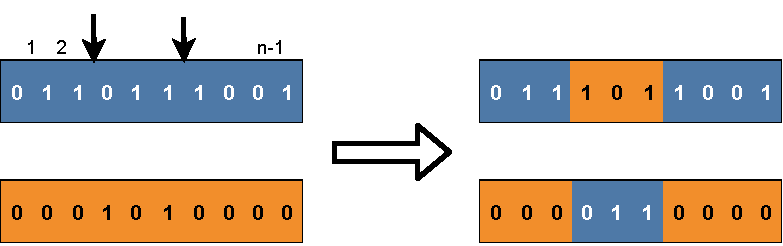
\includegraphics[width=\textwidth]{img/master_twopointcrossover.pdf}
        \caption{Two point crossover}
        \label{fig:gatwopointcrossover}
    \end{subfigure}
    \hfill
    \begin{subfigure}[b]{0.4\textwidth}
        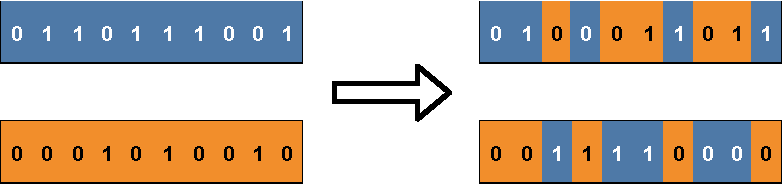
\includegraphics[width=\textwidth]{img/master_uniformcrossover.pdf}
        \caption{Uniform crossover}
        \label{fig:uniformcrossover}
    \end{subfigure}
    \caption{Advanced crossover operators}
\end{figure}

Sometimes, the crossover operator is generalized even more and forms $k$--point crossover. The genotype partitions into $k$ parts and these parts are interleaved in the offsprings. Special case is uniform crossover\index{crossover!uniform} -- the offsprings are constructed in such a way that they are uniform combination if their parents. Each gene in the offspring have equal probability whether it will be received from the first, or second parent. Second offspring will follow the same pattern, except with parents exchanged. Example of uniform crossover is in figure \ref{fig:uniformcrossover}.
% TODO Introduction into GA presents few more types - three parents crossover, crossover with reduced surrogate, and shuffle crossover. These are irrelevant for my implementation, but can be potentially described here.

I have described the crossover operators such that the offsprings replace their parents. That is a common design decision, however one does not need to enforce that and may decide to create offsprings in addition to the parents. To ensure the population does not increase in size, the selection operator can be implemented in a way that specified number of individuals will be picked up.

%%  SELECTION  %%
%%%%%%%%%%%%%%%%%
\subsection{Selection operators}


\chapter{GPU Programming}
Moore's law has driven the rise of processor performance for a long time -- \enquote{The complexity for minimum component costs has increased at a rate of roughly a factor of two per year. Certainly over the short term this rate can be expected to continue, if not to increase. Over the longer term, the rate of increase is a bit more uncertain, although there is no reason to believe it will not remain constant for at least 10 years} \citep{MooresLaw}. This \enquote{law}, if we may call it that way, is unfortunately limited by the physical properties of components used within modern processors. These borders are both on the side of possible processing speed, as well as limited by the size and quantity of transistors in the processor core. Over the last years, scientists are predicting the end of Moore's law \citep{MooresLawEnd}, and their voices are more turbulent since the size of transistors in the \acrfull{acc:cpu} reached $7nm$ in 2018 \citep{SamsungSevenNm}. 

Processor manufacturers are well aware of the physical complications stemming from the transistors' small size and invest more effort into multi--core processors. These processors have many independent cores that can be utilized in parallel and can possibly increase the processor's performance linearly in respect to the number of cores. To name a few, last server processors by Intel\textsuperscript{\textregistered} Xeon\textsuperscript{\textregistered} Platinum 8380 Processor with 40 cores and 80 threads \citep{IntelXeonPlatinum}, as well as AMD EPYC\texttrademark\ 7763 with 64 cores and 128 threads \citep{AMDEpyc}, are great example.

\acrfullpl{acc:gpu}\index{GPU} takes this idea of multi--cores processors further. Rather than increasing single--thread performance, the \gpu manufacturers are concentrating on massive parallelism using a vast number of cores operating in highly parallel and distributed manner \citep{GPUComputingOwens}. Using this strategy, the \gpu programming offers encouraging performance for heavy workloads. Common consumer \acrshortpl{acc:gpu} can easily outperform current high--end \acrshortpl{acc:cpu} in the instruction throughput and memory bandwidth. These demands came originally from the game industry, which places great emphasis on parallel processing and reasonably real--time latency.

The decisions regarding the architecture, though, affect the way \acrshortpl{acc:gpu} are programmed. Unlike \cpu, which can run generic code, \gpu is more suited for specific classes of algorithms that can fully utilize the underlying hardware. Engineers recognized the following mandatory properties of the efficient application running on \gpu \citep{GPUComputingOwens}:
\begin{itemize}
    \item \textit{Large computation demands} -- \gpu can deliver tremendous performance but may weaken it for short tasks without sufficient data. The overhead of memory allocation on \gpu and moving it between can quickly outweigh the advantage of using it. On the contrary, the real--time rendering requires hundreds of operations per pixel, and \gpu can easily meet these demands. \gpu is furthermore hiding memory access latency behind more computations; it needs therefore sufficient work to do that.
    \item \textit{Significant parallelism} -- the algorithm needs to be easy to parallelize and ideally scale to as many cores as possible. Whereas \cpu provides tens of cores (up to 64 today), the \gpu have hundreds or thousands of them (current cutting-edge \gpu produced especially for \acrshort{acc:ai}, NVIDIA V100, has 5120 CUDA cores \citep{nvidiav100spec}), although with limited per--core performance. If an algorithm can employ only a few of them, it may be slower than on multi--core \cpu. Once again, real--time rendering can render each pixel independently, making it a perfect candidate for \gpu computing.
    \item \textit{Throughput over latency} -- because the \gpu is highly parallel by design, the throughput is more important than the absolute latency of individual operations. From the point of rendering, the human eye can perceive images in order of milliseconds. Operations in modern processors take in the order of nanoseconds. Therefore, the absolute time to render a single pixel is not relevant as long as the whole picture is rendered in the same order of time. The algorithms cannot make assumptions about the running time of individual parts but rather on the task's running time as a whole.
\end{itemize}

\acrlong{acc:ea} fits well into these categories, as the algorithm may evaluate individuals' fitness in parallel, and the evaluation is independent in respect to the rest of the population. The crossover and mutation operators may be easily parallelized as well, as they operate and individuals (or a small set of individuals) independently. We may parallelize the algorithm even more by processing each gene separately, as presented by \citet{CHENG2019514}. I will discuss this option at the end of this chapter.




%%%%%%%%%%%%%%%
%%           %%
%%  HISTORY  %%
%%           %%
%%%%%%%%%%%%%%%
\section{History}

Historically, \gpu came from the demand of the game industry for real--time rendering. In the rendering process, a list of geometric primitives, usually triangles, is processed through a number of stages to produce a final picture. The primitives can be processed independently and therefore in parallel, which makes real--time rendering the ideal case for the application of \gpu. The typical operations in graphics consists of \citep{GPUComputingOwens}\index{rendering pipeline}:
\begin{itemize}
    \item Vertex stage that transforms and calculates properties per vertex. Typical operations are transforming vertex position from world space (that is, the coordinates in the scene) into screen space (that is, the coordinates in respect to the viewer point of view) and estimating additional vertex properties like color, material, or texture coordinates.
    \item Primitive assembly transforms geometric primitives into triangles -- the standard geometric primitive for \gpu to work with. This stage may also clip the primitives that are not in the observer's view and save some computation in the following stages.
    \item Rasterization takes generated triangles and resolves which pixels correspond to the provided triangle. These pixels do not necessarily need to match the number of pixels of the screen. They are usually referred to as fragments -- for example, the superscaling technique renders the scene in higher resolution and then downsample it to match screen resolution \citep{GameGraphicProgramming}. Each triangle may be composed of hundreds or thousands of fragments. Moreover, the rasterization typically interpolates vertex properties between the fragments.
    \item Fragment stage processes each fragment and typically resolves the final appearance of the fragment. It may calculate fragment interactions with the lights in the scene, fetch colors from textures, blend fragments, etc. This stage is usually most demanding, as a typical scene consists of millions of fragments.
    \item Composition stage assembles all the fragments into a final image. It may, among others, test fragments visibility, depth, and stencil filter.
\end{itemize}

The stages \gpu performs usually referred to as \emph{rendering pipeline} and may slightly differ. In the beginning, the stages discussed earlier have been preprogrammed by the manufacturer, and developers had only limited options on how to control the pipeline stages (also known as the fixed--function pipeline). As the software complexity increased, the need for more control arise, and the manufactures provided a way to program the individual stages of the pipeline. These programs are called \emph{shaders} and their capabilities matured over the years. In 2006, Microsoft introduced Shading Model 4.0, which allowed using the same programming interface and hardware both for vertex and fragment shader \citep{DirectX10}. Not only that, but more stages appeared (like tessellation and geometry shaders) to provide developers more control over the pipeline. Today, two major \acrfull{acc:api} exists -- proprietary  DirectX and open--source OpenGL. Note that some stages of the rendering pipeline, such as primitive assembly, rasterization, and composition, are still implemented by the \gpu manufacturers and, in most cases, are implemented by special--purpose hardware components (because of the performance reasons) \citep{SoftwareRasterization}. They are, hence, integral components of the rendering pipeline and are not possible to modify.

Soon, scientists and engineers recognized many more problems suitable for processing on \gpu. Although some stages of the rendering pipeline were fully programmable, the pipeline was still inherently graphical, and some stages were not possible to skip. To run general--purpose programs on \gpu required encoding the problem in the domain of geometric primitives and use available programmable and special--purpose hardware to implement the algorithm. Moreover, the programmers need to decide which part of the hardware will execute which part of the calculation and how the pipeline's fixed stages will affect the data structure. As shader programs do not have access to shared memory, the data passing was realized using textures, vertices, and fragment properties \citep{GPUComputingOwens}. These difficulties discouraged general use of \gpu for general--purpose programs, although some efforts have been made to hide the underlying rendering pipeline from the programmer point of view \citep{BrookGPU}.

Lack of support for general--purpose program on \gpu inspired companies to develop a new approach that would provide programmers better control over the underlying hardware. In 2006, NVIDIA introduced first version of \acrfull{acc:cuda}\index{CUDA} \citep{CUDAwiki}. Open--source standard of general--purpose \gpu programming came in 2008 as Open Computing Language (OpenCL) by Khronos Group \citep{OpenCLRelease}. These are higher--level interfaces with C--like syntax exposing \gpu resources without any connection to the graphical pipeline. Programmer is given control of execution and parallelization of the program, as well as memory access. Over the years, these technologies undergo various improvements (the current version is CUDA 11.2, respectively OpenCL 3.0), adding support for data types, language constructs, and new hardware.

\cuda become de facto standard in the field of general--purpose computing on \gpu and I will focus essentially on it. Fortunately, other technologies like OpenCL have alike underlying architecture and approach to the \gpu programming. The following section should hence generalize for them as well.




%%%%%%%%%%%%%%%%%%%%
%%                %%
%%  ARCHITECTURE  %%
%%                %%
%%%%%%%%%%%%%%%%%%%%
\section{Architecture}

The design goal of \gpu is to provide in orders of magnitude higher instruction throughput and memory bandwidth compared to \cpu. The overall architecture of \gpu is therefore significantly different. This section will focus on \gpu architecture from the point of \cuda platform, taking inspiration mainly from the CUDA Programming Guide \citep{CUDAguide}.

\begin{figure}
    \begin{subfigure}[t]{0.47\textwidth}
        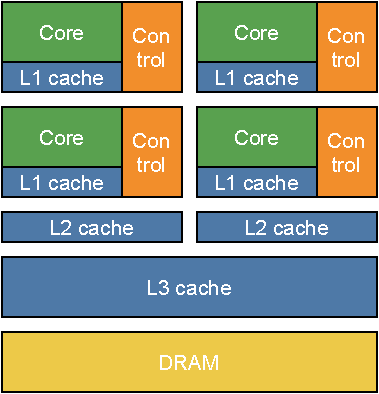
\includegraphics[width=\textwidth]{img/master_cpu_arch.pdf}
        \caption{Architecture of \acrshort*{acc:cpu}. Each core has L1 cache and own control circuit. Cores can therefore work independently.}
        \label{fig:cpuarch}
    \end{subfigure}
    \hfill
    \begin{subfigure}[t]{0.47\textwidth}
        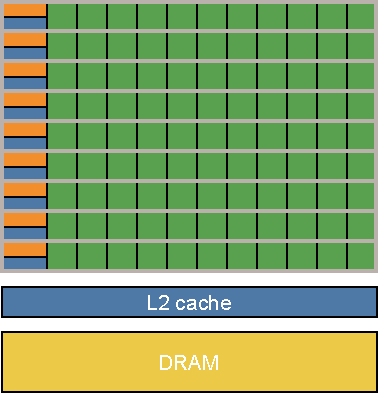
\includegraphics[width=\textwidth]{img/master_gpu_arch.pdf}
        \caption{Architecture of \acrshort*{acc:gpu}. One control circuit controls number of cores. One row of cores is called \acrlong{acc:sm} (\acrshort{acc:sm}, bounded by gray borders). L2 cache is shared between the cores.}
        \label{fig:gpuarch}
    \end{subfigure}
    \caption{Difference between \acrshort*{acc:cpu} and \acrshort*{acc:gpu} architecture}
\end{figure}

The computation power of \gpu emanates from the point that it dedicates more transistors on the chip to the data processing rather than to the control circuitry. The architecture of the \cpu is shown in figure \ref{fig:cpuarch}. Each core has its own control circuit, and therefore each core can execute instructions independently. Moreover, each thread has its own L1 cache.

The \gpu\index{GPU architecture} architecture is portrayed in figure \ref{fig:gpuarch}. A set of cores share the same control circuitry and L1 cache. One line of these cores is called \acrfull{acc:sm}. The exact number of cores per \acrshort{acc:sm} differ between architectures; more information can be found in the article by \citet{NVIDIAhistory} or on NVIDIA official websites. Using one control circuitry to manage many cores brings some implications -- all the cores need to administer the same instruction at once. In this sense, the instruction throughput is achieved using \acrfull{acc:simd} approach -- one instruction can at one tick alter multiple data.

Each \gpu comes with a different set of hardware and software features. Compute capability\index{CUDA!compute capability} specify which features are available on the target system. For example half--precision float--point operations are available from compute capability 5.3. The number of arithmetic CUDA cores per \acrshort{acc:sm} is 8 for compute capability 1.x, 32 resp. 48 for compute capability 2.0 resp. 2.1, 64 for compute capability 6.0, 7.x, and 8.0, 128 for compute capability 6.1, 6.2, and 8.6, and finally 192 for compute capability 3.x. I will not discuss specific compute capability in the following text. I will assume compute capability of at least 6.0 through this work, but I do not depend on the concrete version, as they should be backward compatible. In order to use newer compute capabilities, the \gpu, driver, and the software need to support them.

\acrlong{acc:cuda} allows almost direct translation of code from C onto the \gpu. It uses \cpp language with a few extensions. It is therefore straightforward to write a program for \gpuns, as long as we are familiar with C syntax. To distinguish code running on \cpu and \gpu, \cuda differentiate between host (the code running on \cpu) and device (the code running on the \gpu) functions. There is a particular type of function called \emph{kernels}\index{CUDA!kernel}, which is evoked by the host but executed on the device.

The \cuda defines the following terminology:
\begin{itemize}
    \item CUDA thread\index{CUDA!thread} is execution of a single kernel. To process $K$ blocks of data, the runtime creates at least $K$ threads and runs the same kernel function on each of them.
    \item CUDA thread block\index{CUDA!block} is a collection of threads grouped into the grid. The programmer may specify the size of the grid during the call of the kernel function as a three--dimensional vector. The maximum number of threads in the thread block is limited by the compute capability of the hardware. Moreover, all the threads in the thread block need to be executed on one \acrshort{acc:sm} (with some exceptions) and can be synchronized using \textit{\_\_syncthreads} call. Each kernel receives \textit{threadIdx} variable, which allows identifying individual threads in the block.
    \item CUDA kernel grid\index{CUDA!grid} is a grid of thread blocks. Similarly to thread block, its size may be specified during kernel invocation, and each thread receives \textit{blockIdx} resp. \textit{blockDim} variables identifying block in which the thread is running, resp. size of the blocks. More blocks from the same grid may run in parallel on different or same \acrshort{acc:sm} (if the \acrshort{acc:sm} have free capacity), but the threads from distinct blocks cannot be synchronized.
    \item Warp\index{CUDA!warp} is a set of 32 threads (for all compute capabilities so far) that execute the same instruction. The thread block is split into warps and executed by the \acrshort{acc:sm}. The warp is the minimal unit executable on the \gpu. The device plan warps the same way \acrshort{acc:os} plans processes and may switch context to another warp while the current one is waiting for the data. By executing different warp, the latency of, for example, memory access is \enquote{hidden} behind the execution of different warp. Although \gpu cannot execute anything smaller than the warp (like a single core), it may mask some threads from the execution. Therefore, it is possible to have a block size of $50$ threads; however, $2\cdot32 - 50=14$ cores in the second warp will still execute (although this matter is hidden from the programmer).
\end{itemize}

Because \cuda assumes a system composed of host and device, each of them has its own separate memory. The kernel is executing on the device and, as such, needs to have data its operating moved into the device memory. \cuda provides a set of functions to allocate, deallocate, copy, and move memory between the host and the device\index{CUDA!memory management}. Similar to traditional \cpp programming, \cuda memory is allocated in a single unified linear address space. It can reference other addresses using pointers and use advanced data structures like linked lists and trees. Yet, the data movement between host and device is time--consuming, because the bandwidth between \cpu and \gpu is lower than memory transfers within the device memory. The copy memory from the host to the device may generate nontrivial overhead that may waive the advantage of using \gpu altogether, especially for small kernels. 

To reduce access latency to global device memory, \cuda provides a set of tools to speed up the process. It is possible to control the L2 cache policy to better match executing kernels. It also provides functions to manage \emph{page--locked host memory}, which remains in the host memory and will not page by the \acrshort{acc:os}. Copying from this kind of memory can be done asynchronously, or when allocated as \emph{mapped--memory}, it is shared between the host and the device. Mapped--memory is implicitly transferred to and from the device, and the programmer does not need to allocate it explicitly.

A special kind of memory, residing on--chip, is \emph{shared memory}\index{CUDA!shared memory}. The latency of shared memory is roughly 100x times lower than for global device memory, and the memory is shared in the thread block. Simple operations like matrix multiplication can hasten by order of magnitude using shared memory \citep{MatrixMultiplicationGPU}. However, shared memory operates in equally--sized memory modules called banks, which complicates concurrent access to the shared memory. All the compute capabilities up today have 32 banks for shared memory organized into 32--bit words. Access to distinct memory addresses belonging to the same bank (bank conflict) by multiple threads within the same warp is serialized and, therefore, significantly increases the kernel's running time. This is common for data types with 64--bits, such as double--precision floats. It may be beneficial to pad each value with one byte to eliminate conflicting access to the same banks.

As I mentioned earlier, all threads in the warp need to execute the exact same instruction. However, the programming language supports conditional jumps, loops, and other constructs known from the modern programming languages. It may certainly happen that some threads within the warp may execute different execution path -- a situation known as \emph{warp divergence}\index{CUDA!warp divergence}. There are further causes, why the threads in the warp may diverge, but the branching is the most common one. In order for \gpu to evaluate each execution path, it executes the branched paths sequentially and masks out threads not participating in the current one. Masked threads will execute the program; however, their results are ignored from the programmer point of view. This implies the same code will be executed twice (note that this grows exponentially for nested conditions) and significantly extend the time to finish the program. In general, warp divergence is undesirable and should be avoided when possible.
Warm divergence can only occur within a warp. Different warps in the same thread block may execute different execution paths without any impact on the program's performance.

The parallel nature of \cuda supports several algorithms that have by order of magnitudes better performance on \gpu than on \cpuns. A typical example would be element--wise linear operations or matrix multiplication \citep{GPUMatrixMultiplication}. Reduction operations such as summation of the array can be implemented effectively on \gpu \citep{harris2007optimizing}, as well as different kinds of sorting algorithms \citep{GPUsorting}.

These operations are so popular, NVIDIA released a set of libraries with the implementation of these algorithms. The most relevant for this work are \textit{cuBLAS} (GPU--accelerated basic linear algebra library), CUDA Math Library implementing most common mathematical functions, and \textit{cuRAND} (GPU--accelerated random number generation). These implementations are optimized for the latest hardware and maintained by NVIDIA.




%%%%%%%%%%%%%%%
%%           %%
%%  PYTORCH  %%
%%           %%
%%%%%%%%%%%%%%%
\section{PyTorch}

From the brief description of \cuda above is clear that programming in \cuda is fundamentally different from programming in traditional programming languages like C or \cppns. The efficient implementation of kernels is complex, and in order to fully use the power of \gpuns, the programmer needs to understand the underlying hardware. Not an ability commonly found among scientists and engineers dealing with evolutionary algorithms. As one of the goals of this thesis is to provide easy--to--use and extend library for evolutionary algorithms, I decide to look for an alternative.

PyTorch\index{PyTorch} is free open--source library maintained by Facebook's AI Research lab (\href{https://ai.facebook.com/}{FAIR}). It builds on top of \href{http://torch.ch/}{Torch} library for scientific computing on \gpuns. It is possible to use \cpp or Python programming languages to implement applications using PyTorch library, where the Python language is the primary language the library focuses on. I argue that more programmers are familiar with Python language than with C or \cppns; and its use is hence more plausible than \cuda for my purpose \citep{StackOverflowSurvey}. PyTorch hides the underlying kernels behind a unified interface, and the programmer does not need to know \cuda programming at all. When necessary, PyTorch allows to implement parts of the algorithm in \cpp or even as a native \cuda kernel and chain it with the rest of the PyTorch library \citep{PyTorchDoc}. The end--user may call this native implementation directly from Python source code without noticing it. This approach allows optimizing specific parts of the algorithm if the performance is not pleasing.

The building block of PyTorch library is the \incode{torch.Tensor} data type\index{PyTorch!data types}. It represents a multidimensional array of scalars. PyTorch allows to define the type of the scalars to be the same as supported by most of the programming languages, the most common are 16,32, or 64--bit floating--points numbers (also known as half--precision, single--precision, and double--precision floating--point formats), signed 8, 16, 32, and 64--bit integer numbers (also known as char, short, integer and long numbers), 8--bit unsigned integer (known as byte), and Boolean data type storing either 1 (true) or 0 (false) values. Except for these, PyTorch supports 32, 64, and 128--bit complex numbers.

Tensors are efficiently stored in memory by setting the size and stride of each dimension. This allows representing $k$--dimensional tensor of constant value by only a single value in memory. We set the desired size of each dimension and stride equal to $0$. Because PyTorch kernels anticipate tensors in this format (with size and stride defined), they will automatically reference the single value instead of duplicating it in the memory. There is also the possibility to store sparse tensors using the \incode{torch.sparse} package and keep in memory only non--zero values. Note that sparse tensors are only in beta \citep{PyTorchDoc}.

The kernels are realized as operations with tensors\index{PyTorch!operations}. PyTorch provides a broad range of operations, highly similar to the functions in the NumPy library, which is de facto standard for numeric computation algorithms in Python. These functions are also similar to MATLAB numerical functions, and very presumably, programmers coming from other platforms may effectively implement their algorithms in PyTorch because the \acrshort{acc:api} is familiar for them. This is one of the reasons why I choose PyTorch as the library for the implementation of evolutionary algorithms.

PyTorch functions realize standard algebraic operations, geometric and statistical functions, matrix multiplication, bitwise operations, reduction operations like summation, finding unique elements, or logical testing of the list of variables. Moreover, PyTorch implements functions from BLAS (Basic Linear Algebra Subprograms) specification and LAPACK (Linear Algebra Package) library like matrix decomposition, linear equations solver, determinant, and much more \citep{PyTorchDoc}.

For pseudo--random number generation uses PyTorch underlying implementations -- either Mersenne Twister for CPU or Philox implemented in NVIDIA's cuRAND library. The latter is efficient for \cuda programming and does not make a major challenge. Historically, people were generating random numbers on \cpu and moving them to \gpu afterward. Using native \cuda implementation is by no means more effective.

The advantage of PyTorch is that its functions are implemented both for \cpuns, as well as for \gpuns. It is possible to use the same source code without any changes on machines without \gpuns. The implementation may still use \acrshort{acc:simd} instructions on \cpuns, that are ordinarily available on modern processors (also known as vectorized instructions). Note that although these are still \acrshort{acc:simd} instructions, the performance is not nearly as good as running all the computations on \gpu in parallel. Nevertheless, the performance would still be a bit better than using C or \cppns purely.

Another advantage of using an existing library like PyTorch is that the implementation (and especially the \cuda kernels) is written and maintained by a team of professionals that understand the architecture and working of the \gpu most likely better than most of the people dealing with evolutionary algorithms. Using existing frameworks gives assurance the kernels are implemented efficiently both on the \gpu and \cpuns. What is, in my opinion, more important is that the library is kept up--to--date and may use features of new, not yet released hardware, in the future. All we need to do is to update the library, and the same source code may use the new hardware and features.

Because of the PyTorch properties mentioned above, I decided to implement the evolutionary algorithms in this framework.




%%%%%%%%%%%%%%%%%%%%%%%%%%%
%%                       %%
%%  EVA PARALLELIZATION  %%
%%                       %%
%%%%%%%%%%%%%%%%%%%%%%%%%%%
\section{Evolutionary Algorithms parallelization}

General \acrlong{acc:ea} manage a population of individuals and by repeated application of evolutionary operators search for the optimal solution of the problem in hand. As the individuals within the population are independent, there is excellent potential to speed up the whole process by parallelizing evolutionary operators. Although some of the operators need more than one particle for their execution (the crossover operators are the typical example), the operator is, in most cases, applied several times on different sets of individuals. Further, these sets are usually small, and the operator may be executed in parallel for all of them. The typical crossover operator, for example, needs only two individuals and is applied for half of the population.\todo{Polovina je prý divná}

Scientists and engineers were well aware of this potential, and the first attempts to parallelize evolutionary algorithms came long before \cuda was introduced by NVIDIA \citep{PGAPack} in 2006. These projects were either using a single machine with multiple processor cores or a system of machines sharing the population over the network. The common idea is to divide the population into chunks and solve them simultaneously using multiple processors. There are two way of doing that \citep{CHENG2019514}:
\begin{itemize}
    \item Master--worker model executes all the evolutionary operators on a single machine, but the fitness evaluation is spread among several processors. While the fitness evaluation takes a significant amount of time (for example, run of a physical simulation is very time--consuming), and the time to share the individuals among processors is negligible, the master--worker model is the best way to accelerate the algorithm.
    \item Island model maintains a list of populations evolving independently. Each of these populations may run on a separate processor and therefore in parallel. The populations are usually called \emph{islands} because from the evolutionary point of view appear as evolutions on different continents. The islands do not collaborate with each other, except a specific operator called \emph{migration operator}\index{migration operator}. This operator periodically, in a predefined way, exchanges a small portion of the population amidst islands. By borrowing few individuals from a different island, we hope to bring new genetic material. There has been shown that the island model on its own may improve the solution quality and running time of the algorithm \citep{IslandModel}.
\end{itemize}
These models are historically more suited for multi--processor systems rather than for \gpuns, as it would be hard to scale them up to thousands of cores currently available in modern \gpuns. Nevertheless, these approaches can still be combined with the proposed implementation. One may, for example, use the island model and run each population on a different \gpuns--enabled machine.

\begin{figure}[hb!]
    \centering
    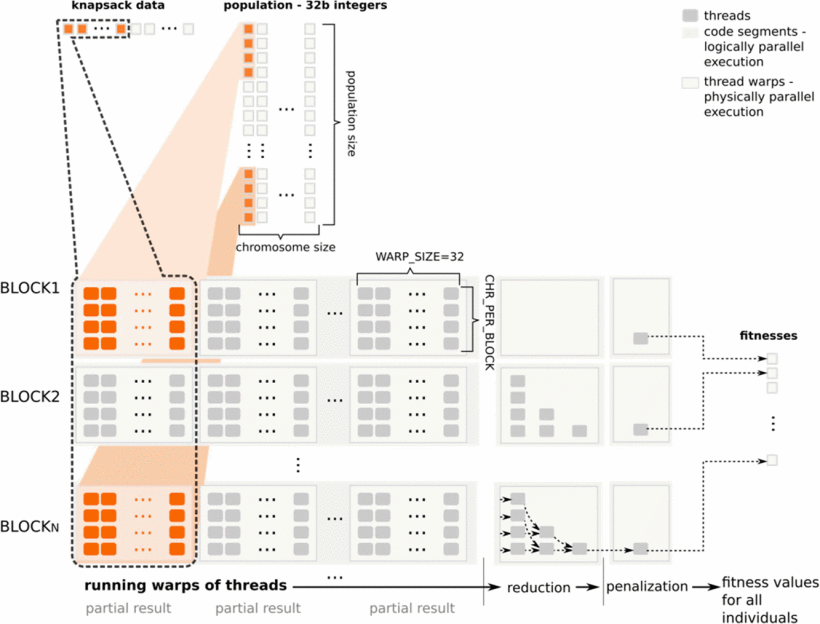
\includegraphics[width=0.8\textwidth]{img/KnapsackKernelDesign.png}
    \caption[Knapsack problem CUDA evaluation kernel]{Design of the knapsack fitness function kernel in \citet{GpuIsland}. It is gene--level model, where each thread aggregate informations from one individual and $CHR\_PER\_BLOCK$ items.}
    \label{fig:knapsackkernel}
\end{figure}

In parallel computing, the granularity\index{granularity} is a measure of the computation amount conducted by the task. Typically there is coarse--grained parallelism, which splits the problem into several large tasks. Fine--grained parallelism, in contrast, breaks the problem into a large number of small tasks. Both coarse--grained and fine--grained algorithms have been proposed for \cpu architecture. For \gpu programming, however, more delicate levels of granularity are needed:
\begin{itemize}
    \item Chromosome--level granularity evaluate one individual using one thread. Master--worker model mentioned earlier is an example of the chromosome--level granularity. For \cuda purposes, this degree of granularity is still too raw.
    \item Warp--level granularity evaluate one individual using warp of threads. The advantage of warp is that threads within may communicate, and for some problems, this may be necessary to do so.
    \item Gene--level granularity evaluate each gene using one thread, or more generally evaluate one individual using more threads (then warp--level granularity is just a special case of the gene--level granularity).     
\end{itemize}
The gene--level granularity is ideal for the \gpu computing, as it exposes enough parallelism. Earlier attempts with chromosome--level or more coarse level granularity could not fully utilize the \gpuns. One example of the gene--level granularity is in the work of \citet*{GpuIsland} for the knapsack problem. His design of the \cuda kernel is in the figure \ref{fig:knapsackkernel}. Other author implemented various algorithms using \cudans, for example, simple genetic algorithm \citep{SimpleGACUDA}, differential evolution \citep{veronese2010differential}, and particle swarm optimization \citep{PSOCUDA}. All of them showed in the order of magnitude speedup and proof that implementing \acrlong{acc:ea} on \gpu has its advantages.

\chapter{Proposed implementation}
\label{chap:impl}

My goal is to design and implement library for \acrlong{acc:ea}, as mentioned in the chapter \ref{chap:intro}. The library should not only implement existing \acrshortpl{acc:ea} and allow to execute them on the \gpuns, but also afford a general framework to which it would be simple to plug new algorithms. For the user of the library should be easy to replace evolutionary operators, modify them, or, if necessary, replace the whole workflow of the algorithm.

I decide to implement the library using Pipe and Filter architecture as specified by \citet{EnterpriseIntegrationPatterns}. The example of this architecture is in figure \ref{fig:pipesandfilters}. The general idea is to partition the algorithm into smaller, simple steps and use the output of one step as the input to the following one. \acrshort{acc:ea} are simple to split, as one step may be one evolutionary operator. I decided to implement the library in the \enquote{Convention over Configuration} design pattern -- that is, the operators make the same assumptions about the format and order of the input, rather than explicitly specifying it in the configuration. I still provide ways to control the order of parameters, if required by the user, and I will get to it a bit later.

\begin{figure}
    \centering
    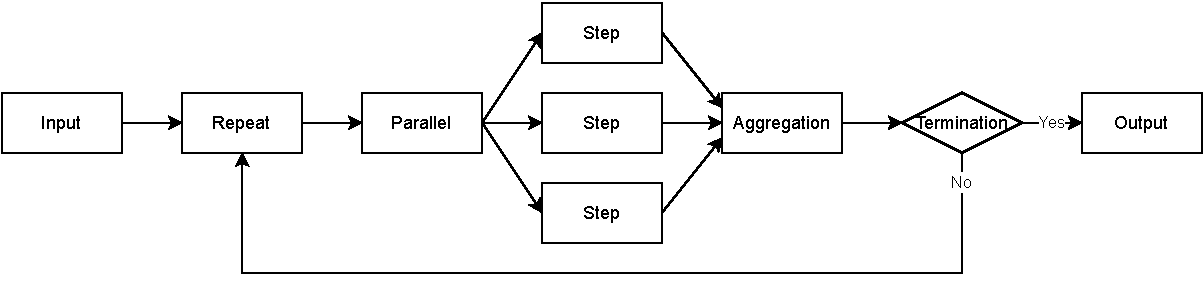
\includegraphics[width=\textwidth]{img/PipesAndFilters.pdf}
    \caption{Pipe and Filter architecture}
    \label{fig:pipesandfilters}
\end{figure}

The pure Pipe and Filter architecture is not sufficient for implementation of \acrshort{acc:ea}. In the purest implementation, this architecture is just a chain of steps following each other. I decided to expand it by numerous practical steps like loops, parallel step invocation, and more. An example of parallel step respectively loop used in the Pipe and Filter architecture is demonstrated in figure \ref{fig:pipesandfilters}. The parallel invocation is depicted in the figure by \enquote{Parallel} block, followed by the \enquote{Aggregation} block accumulating the results from each step. The loop is represented by the \enquote{Repeat} block accompanied by the \enquote{Termination} block controlling the termination condition of the loop.

My proposed implementation is the \emph{\acrfull{acc:ffeat}}. This library is attached to this work, available on my GitHub account \citep{FFEATrepo}, and ready for install as PyPI (Python Package Index) \href{https://pypi.org/project/FFEAT/}{package}. The PyPI is de facto standard way of installing Python packages from a central repository.

As I mentioned earlier, I decided to implement the library in the Python programming language and using PyTorch library. Python allows invocation of function with a variable number of arguments and a variable number of keyword arguments. Without explaining it in too much detail, arguments are passed into the function in a list and depend on their order. These are the traditional arguments known from languages like C and \cppns. Keyword arguments must be specified by their parameter name. The following line of code invokes function \textit{some\_function} with two parameters $1$ and $2$, and a keyword argument $karg=5$.

\begin{lstlisting}[language=Python]
some_function(1, 2, karg=5)
\end{lstlisting}

I use this design to implement operators in Pipe and Filter architecture. The operator accepts a variable number of normal and keyword arguments and returns a list of variables and a dictionary. The list of variables, respectively the dictionary serves as the input for the following operator as normal, respectively as keyword arguments. Following this design, a new operator may be easily plug\-in into the algorithm. At the same time, it allows using the same underlying architecture both for genetic algorithms (the argument is only the population), as well as \acrshort{acc:pso} algorithms (using particles' position, velocity, and their best--known positions as three distinct arguments).

The library expects the population to be represented as the tensor, respectively, as a list of tensors, where the first dimension enumerates over the individuals (note that the tensor needs to be aligned in each dimension). I resolve to this assumption because it allows me to implement the operators more efficiently. Nevertheless, the architecture is general enough, and it may easily adjust to the problem at hand; the user would just need to reimplement the operators where necessary. In most cases, it is enough to represent the population using a single, two--dimensional tensor. Some operators are implemented in a way, they may handle multi--dimensional tensors as well (for example uniform crossover). In the case of \acrshort{acc:pso} algorithm, using a single tensor is not sufficient. The library represents the swarm using a list of tensors -- one tensor for each component of the population. Specifically, the library creates tensors: particles' position and velocity, local and best--known positions, and their corresponding fitness values. Although the \acrshort{acc:pso} uses list of tensors, each of them still fulfills the requirement to use the first dimension to enumerate over individual particles. The operators can hence effectively run in parallel.

The library is split into several modules, focusing on different kinds of evolutionary algorithms or solving particular problems.
\begin{itemize}
    \item \incode{ffeat.flow} module includes basic classes to control the flow of the algorithm with the Pipe and Filter architecture in mind.
    \item \incode{ffeat.genetic} implements genetic algorithms operators and assume binary encoding.
    \item \incode{ffeat.strategies} contains all the real--coded operators. Although not all of them are adaptive, therefore, cannot be considered as evolution strategies, I decided to put them into the shared module for convenience.
    \item \incode{ffeat.pso} handles \acrlong{acc:pso} algorithms, their neighborhood and velocity update algorithms.
    \item \incode{ffeat.measure} implements aggregations functions, primary focusing on fitness metrics.
    \item \incode{ffeat.utils} is a support module containing various useful functions like fitness scaling, decay, and early termination implementations.
\end{itemize}

The base class for all the operators is \incode{ffeat.Pipe}. The implementation merely accepts all the arguments and returns them. The specific logic needs to be provided by the derived class. The method the library invokes is the Python's \incode{__call__} method allowing call the object the same as it was a function. That means the library invokes the operators using the standard invocation procedure, allowing the implementation of simple operators by a function or a lambda function rather than a class.

The \incode{ffeat.flow} implements basal classes to use the Pipe and Filter architecture. I will refer to operators to invoke as \enquote{filters} to agree with the architecture naming. The most important filters are:
\begin{itemize}
    \item \incode{Sequence} executing filters in sequence and passing the output of the preceeding one into the following. The \incode{Sequence} class implements the simplest Pipe and Filter architecture alone.
    \item \incode{Parallel} executes filters in parallel -- that means all of them receive the same parameters, and their results are concatenated together. The execution is parallel from the logical point of view, not using multithreading.
    \item \incode{Repeat} executes filters in a loop for a given number of iterations (or indefinitely). The implementation allows breaking the loop early by passing \enquote{break} parameter as a keyword argument into the inner filters.
\end{itemize}
The module encompass few more classes allowing to reorder and discard parameters (\incode{Select} class), replace some of them (\incode{Replace} class), transform each parameter (\incode{EachArg} class), and use Python lambda function (\incode{Lambda} class). I do not want to discuss them here, as the details are no important. Please see the attached source code for more information.

Before I describe particular operators, I would like to discuss the limitations of the PyTorch library and \gpu programming in general. As I already mentioned in chapter \ref{chap:gpu}, the most costly situation is swarm divergence. I tried to implement all the operators without condition statements and, therefore, eliminate the swarm divergence situation as much as possible. I found boolean mask maps as a suitable replacement for condition statements. PyTorch allows using a boolean mask either for indexing (if the only portion of tensor should be updated) or in an arithmetic operations by multiplying tensor by the mask (and zeroing portion of the tensor).

A further limitation is the \gpu memory, which is a scarcer resource in comparison to the servers. Modern graphical cards have up to small dozens of GB of memory (the latest NVIDIA V100 has 32GB \citep{nvidiav100spec}), whereas modern servers have hundreds of GB of memory. Because the library may use vast populations, even memory reallocation may be problematic, as the whole population must fit into the memory at least twice. I decided to implement the operators in--place, that is, all the operators are applied on the same memory. Not only it uses less memory, but it is also more efficient. For some operators (typically crossovers) is still possible to opt--out of in--place mode (for example, in the case of plus or comma crossover schema).

Some operators, for example crossovers and differential evolution, should receive distinct parents in order for the operator to do something useful. Unfortunately, this requirement is hard to satisfy, especially for \gpuns, because the parent indices are generated independently. It is, nevertheless, still possible using PyTorch's \incode{torch.multinomial} function. The problem is, this function is significantly costly and takes in order of magnitude more time than generating a random integer in a given range. I decide to allow specification of the parent sampling strategy for all these algorithms.
\todo{Pravděpodobně změřit čas a fitness hodnoty pro obě strategie. Předpokládal bych, že s větší populací je pravděpodobnost duplicity menší a nebude to takový problém. Sem dát stručný popis, že to nevadí, a detailnější rozbor udělat v další kapitole.}



%%%%%%%%%%%%%%%%%%%%%%%%%%
%%                      %%
%%  GENETIC ALGORITHMS  %%
%%                      %%
%%%%%%%%%%%%%%%%%%%%%%%%%%
\section{Genetic Algorithms}

The \acrlongpl{acc:ga} are in the \incode{ffeat.genetic} module. This module is further divided into following submodules.
\begin{itemize}
    \item \incode{ffeat.genetic.initialization} holds classes initializing the population. I considered only random initialization of individuals for the \acrshort{acc:ga} case, and this is implemented by the \incode{Uniform} class.
    \item \incode{ffeat.genetic.evaluation} submodule contains classes to evaluate the individuals. The \incode{Evaluation} class expect to evaluate the whole population at once (ideal for \gpu implementation), whereas the \incode{RowEval} evaluate individuals one after another. Both classes expect fitness function during their creation.
    \item \incode{ffeat.genetic.mutation} includes mutation operators. The library only implements simple Flip--Bit mutation operator, allowing to specify number of mutated individuals and probability of gene change.
    \item \incode{ffeat.genetic.crossover} submodule.
    \item \incode{ffeat.genetic.selection} submodule.
\end{itemize}

I implemented uniform, one--point, and two--point crossovers for \acrshort{acc:ga} (classes \incode{Uniform}, \incode{OnePoint1D}, and \incode{TwoPoint1D}). The uniform crossover may handle individuals with an arbitrary number of dimensions because it simply generates a random mask of genes to inherit from the first parent. For one--, and two--point crossovers would be the position of the crossover point ambiguous; they, therefore, expect individuals to be one--dimensional.
\todo{Rozhodnout jestli psát o implementaci point crossover operátorů na základě měření.}

All the crossover operators implement three distinct schemes of how to handle the offsprings. The default scheme is the in--place version and the offsprings replace their parents. For this to work, the crossover must produce the same number of offsprings as there are parents. Moreover, the crossover operator should not process the whole population, as it may destroy it or shift the whole population into an undesirable region of the search space. Still, I decide to use it as the default version because of the \gpu limitations mentioned above.
The second and third schemes are the comma and plus schemas mentioned on the page \pageref{enum:steadystate}. The plus scheme concatenates the offsprings with the parents and is specified by the \incode{replace_parents=False} argument. The comma scheme returns just the offsprings and is specified by the \incode{discard_parents=True} argument passed to the crossover constructor.

\begin{algorithm}[b!]
    \begin{lstlisting}[language=Python, xrightmargin=18pt]
    import ffeat.genetic as GA
    
    
    fn = create_problem_function()
    
    alg = GA.GeneticAlgorithm(
        # Randomly initialize 100 individuals 
        # with gene of length 40
        GA.initialization.Uniform(100, 40),
        # Evaluate the population
        GA.evaluation.Evaluation(fn),
        # Sample 100 individuals into new generation
        GA.selection.Tournament(100),
        # Crossover 40% of them
        GA.crossover.OnePoint1D(0.4),
        # Mutate 60 of them with 1% mutation chance
        GA.mutation.FlipBit(60, mutate_prob=0.01),
        # repeat for 100 generations
        iterations=100
    )
    alg() # run the evolution
    \end{lstlisting}
    \caption{Simple \acrshort*{acc:ga} in \acrshort*{acc:ffeat}}
    \label{alg:gaffeat}
    \end{algorithm}

In the \incode{ffeat.genetic.selection} module the library keeps implementations of the 
tournament (\incode{Tournament} class)
roulette (\incode{Roulette} class), 
and \acrlong{acc:sus} (\incode{StochasticUniversalSampling} class)
selection operators. The tournament selection allows to specify whether is it maximization or minimization problem and a number of parents, as I discussed in chapter \ref{chap:eva}. The rank--based selection operator is in fact roulette or \acrshort{acc:sus} selection with preprocessing of fitness values. I will get to fitness transformation later.

I also implement elitism in the \incode{ffeat.genetic.selection.Elitism} class. It copies the $n$ best individuals from the population and temporarily stores them aside. After all the \acrshort{acc:ga} operators execute, it copies them back into the population. The implementation does not follow the exact description found in books \citep{IntroductionToEA}, because it may replace better individuals (when the elite improve). The standard implementations of elitism prohibit elites change by the following operators, or append the elites to the population after all the operators are executed. 
Because the operators following the elitism may be arbitrarily complicated, or the user of the library may decide to implement their own set of operators, ensuring the elites would not change would be thorough and delicate work. % TODO jsou would spravne?
From the \gpu programming point of view, copying small amount of memory between already allocated memory space is more efficient than appending the elites to the population, because that would require reallocation of the whole population.
\todo{Možná zmínit, že je malá pravděpodobnost, že se to stane (zdroj?) a nebo že nám to nevadí (měření?) -- to že elita přepíše lepšího jedince. Popřípadě že to zjednodušuje implementaci.}
\todo{Na základě měření diskuze o implementaci.}

For convenience, the parameters dealing with population size, typically the number of individuals to sample during selection, or the number of offsprings in crossovers, can be specified using an absolute number or a fraction of population size. Moreover, some operators' parameters may change between the generations, for example mutation probability of Flip--Bit mutation. These parameters accept callable object evaluated each iteration, allowing them to adjust. Finally, there is no need to use \incode{ffeat.flow} module directly, but the flow is wrap in the \incode{ffeat.genetic.GeneticAlgorithm} class, into which the user just needs to plug the operators.

Example of genetic algorithm in the \acrshort{acc:ffeat} library is in the algorithm \ref{alg:gaffeat}.

\todo{Někam vrazit problémy GPU programování a jak jsme je řešil. Může být spojeno s parental sampling.}

\todo{Přidat ukázky nějakých operátorů.}



%%%%%%%%%%%%%%%%%%%%%
%%                 %%
%%  REAL-CODED EA  %%
%%                 %%
%%%%%%%%%%%%%%%%%%%%%
\section{Real--Coded Evolutionary Algorithms}

Real--coded evolutionary algorithms are encapsulated in the \incode{ffeat.strategies} module. It has similar structure to \acrshort{acc:ga} module described above. Except for the operators mentioned above, I implemented operators specific to real--value encoding.

In the \incode{ffeat.strategies.crossover} submodule is uniform, one--point, and two--point crossovers identical to one for \acrshort{acc:ga}. Besides, it contains:
\begin{itemize}
    \item Arithmetic crossover in the \incode{Arithmetic} class. It allows specifying the number of parents and their weights. For $k$ parents, the offspring is created by the formula 
    $$\mathbf{o}_i=\sum_{j=1}^k w_{ji}\mathbf{p_j}_i$$
    It allows passing a callable object for the weights so that the weights may be randomized and the offspring may be different weighted arithmetic sum each generation (allowing different weights for individuals' genes as well).
    \item Blend crossover in the \incode{Blend} class, as described in the chapter \ref{chap:eva}.
    \item Differential evolution implemented by the \incode{Differential} class. Although this operator may be used alone, I decide to keep it among the crossover operators. It is possible to alter the $F$ and $C$ constants over generations and replace the parent only if the offspring is better than its parent. In this case, the operator needs to know the fitness values of the parents.
\end{itemize}
\todo{Možná něco o implementaci podle toho, jak dopadne měření.}

\begin{algorithm}[b!]
\begin{lstlisting}[language=Python, xrightmargin=18pt]
import ffeat.strategies as ES


fn = create_problem_function()

alg = ES.EvolutionStrategy(
    # Randomly initialize 100 individuals 
    # in range (-5,5) with gene of length 40
    ES.initialization.Uniform(100, -5.0, 5.0, 40),
    # Evaluate the population
    ES.evaluation.Evaluation(fn),
    # Sample 100 individuals into new generation
    ES.selection.Roulette(100),
    # Crossover 40% of them
    ES.crossover.TwoPoint1D(0.4),
    # Use normal mutation for all of them with 
    # standard deviation 0.01
    ES.mutation.AddFromNormal(0.01),
    # repeat for 200 generations
    iterations=200
)
alg() # run the evolution
\end{lstlisting}
\caption{Simple real--coded algorithm in \acrshort*{acc:ffeat}}
\label{alg:esffeat}
\end{algorithm}

From the mutation operators, I implemented the following operators in the \incode{ffeat.strategies.mutation} submodule.
\begin{itemize}
    \item Random replacement of gene by a value sampled from the specified distribution. It supports all the distributions implemented by PyTorch library and may refine the mutation rate over generations \citep{PyTorchDoc}. It is implemented in the \incode{Replace} class, along with the \incode{ReplaceUniform} class sampling from uniform distribution.
    \item Small deviation of the individual by adding value sampled from the specified distribution. It is encapsulated in the \incode{AddFromDistribution} class with specialized classes \incode{AddFromNormal} and \incode{AddFromCauchy} for normal respectively Cauchy distribution. The \incode{AddFromNormal} is the traditional implementation of normal mutation specified in the first chapter.
    \item Normal mutation with adaptive step implemented in the \incode{AdaptiveStep} class. It supports only the simplest adaptive algorithm by sharing the same deviation for all the dimensions. It allows specifying initial, maximal, and minimal deviation, as well as step size and a number of better offsprings needed to increase the deviation. It may be used to implement the one--fifth rule.
\end{itemize}

The \incode{ffeat.strategy.EvolutionStrategy} class wraps together all the steps for real--coded evolutionary algorithms. Simple real--coded algorithm is in algorithm \ref{alg:esffeat}.
    



%%%%%%%%%%%%%%%
%%           %%
%%  UTILITY  %%
%%           %%
%%%%%%%%%%%%%%%
\section{Utility functions}

I implement some functionality allowing to control and measure the algorithm progress. The first set of these functions are in the \incode{ffeat.measure} module. It allows measuring statistical data, like mean, deviation, and quantiles of the population fitness. It passes measured metrics as keyword arguments to the following operator, so it is possible to stop the algorithm early if a specific metric does not improve or a certain threshold has been reached. Also, it is possible to log these metrics into standard output or file, if necessary.

The \incode{ffeat.utils.termination} submodule responsibility is the early termination of the algorithm. There are various termination criteria, for example if metric does not improve for a specified number of generations (\incode{NoImprovement} class), metric deviation for last $k$ is bellow certain threshold (\incode{StdBellow} class), or metric reached specified threshold (\incode{MetricReached} class).

The decay rates presented in section \ref{chap:adaptiveoperators} are implemented in submodule \incode{ffeat.utils.decay} -- specifically the module implemenets linear, polynomial, and exponential decay rates. This module allows, for example, decrease the mutation rate over generations.

Last submodule is \incode{ffeat.utils.scaling}, allowing to rescale the fitness for the purposes of roulette--based selection operators. The fitness may be scaled linearly, exponentially, or using a logarithmic scale. Special transformation is in the \incode{MultiplicativeInverse} class, transforming minimization problem into maximization one by changing fitness by the $f(x)=1/x$ formula.

Earlier in this work, I mentioned that rank--based selection operators are just roulette-based selection operators with modified fitness values. Class \incode{RankScale} conduct that by sorting the population by the old fitness values and giving each individual a new fitness value based on its order. The given fitness values are linearly distributed among the population, but may be transformed into different scale using one of the above--mentioned classes.
\todo{Diskuze nad efektivitou po provedení měření, možná až v další kapitole.}




%%%%%%%%%%%%%%%%%%%%%%%%%%%%%%%%%%%
%%                               %%
%%  PARTICLE SWARM OPTIMIZATION  %%
%%                               %%
%%%%%%%%%%%%%%%%%%%%%%%%%%%%%%%%%%%
\section{Particle Swarm Optimization}

The \acrlong{acc:pso} algorithms are implemented in the \incode{ffeat.pso} module. It contains the implementation of both \acrshort{acc:spso2006} and \acrshort{acc:spso2011} algorithms, along the following neighborhoods in the \incode{ffeat.pso.neighborhood} submodule.
\begin{itemize}
    \item Random neighborhood.
    \item Nearest neighbors neighborhood.
    \item Static neighborhood is a helper class that cache the neighborhood in the first generation and uses it for the rest of the algorithm run. Following neighborhoods use the static neighborhood as their base class, and therefore the time to build the neighborhood does not affect the algorithm's running time.
    \item Circle neighborhood with the possibility to specify the number of neighbors.
    \item Grid neighborhood with either linear, compact, or diamond shape, as specified in chapter \ref{chap:psoneig}. The compact and diamond shapes are tricky to build in an arbitrary number of dimensions, so these are implemented only for two--dimensional cases and encapsulated in the \incode{Grid2D} class.
\end{itemize}

In the \incode{ffeat.pso.clip} submodule are classes allowing to clip either particles' position or their velocity, both per dimension or the by absolute velocity value.

The whole \acrshort{acc:pso} algorithm is wrap inside the \incode{PSO} class. Because of the more complicated flow of the algorithm, this class does not allow as much freedom as previous \acrshort{acc:ga} or real--coded \acrshort{acc:ea} implementations. The example of \acrshort{acc:pso} algorithm in \acrshort{acc:ffeat} is in algorithm \ref{alg:psoffeat}.

\begin{algorithm}[b!]
\begin{lstlisting}[language=Python, xrightmargin=18pt]
import ffeat.pso as pso


fn = create_problem_function()

alg = pso.PSO(
    # Randomly initialize position of 100 particles
    pso.initialization.Uniform(100, -5.0, 5.0, 40),
    # Randomly initialize velocities
    pso.initialization.Uniform(100, -1.0, 1.0, 40),
    # Pass the evaluation function
    pso.evaluation.Evaluation(fn),
    # Specify random neighborhood with 3 neighbors
    pso.neighborhood.Random(3),
    # Use SPSO2006 velocity update rule
    pso.update.PSO2006(
        inertia=0.8, 
        local_c=1.5, 
        global_c=1.5
    ),
    # Clip particles position into range
    clip_position=pso.clip.Position(-5,5),
    # Clip particles velocity
    clip_velocity=pso.clip.VelocityNorm(2.0),
    # Specify number of iterations
    iterations=200
)
alg() # run the PSO algorithm
\end{lstlisting}
\caption{\acrshort*{acc:pso} algorithm in \acrshort*{acc:ffeat}}
\label{alg:psoffeat}
\end{algorithm}

\chapter{Evaluation}

In this chapter, I will begin by introducing testing problems, against which I will evaluate the implementation. The subsequent section describes the hardware specification of the machines I tested the implementation on. The discussion about the results is in the last section with selected measurements. You can see complete results in appendix chapter \ref{chap:results}. The hyperparameters used for these measurements are in appendix chapter \ref{chap:hyperparameters}.




%%%%%%%%%%%%%%%%%%
%%              %%
%%   PROBLEMS   %%
%%              %%
%%%%%%%%%%%%%%%%%%
\section{Problems description}

For the \acrlong{acc:ga} evolution I used \acrshort{acc:sat} and \acrshort{acc:3sat} problems with various number of literals and clauses. The fitness function sums a number of unsatisfied (for minimization problem) or satisfied (for maximization problem) clauses. I implemented the fitness evaluation in a vectorized manner in PyTorch, so the whole population is evaluated at once. I generate a new problem for every new measurement, and all the problems have been satisfiable. I achieved that by generating the first assignment of all the literals and then generating the desired number of clauses. At least one literal in each clause matches the value with his corresponding counterpart in the previously generated assignment. Because I am more concerned with the running time of the algorithm rather than its performance, the satisfiability of the formulas does not make a big impact on the measurements.

The problem formula is kept as a matrix, where rows correspond to clauses and columns to indices of literals in the clause. For a negative literal, the index is negative. This coding is efficient for \acrshort{acc:3sat} problem, but I run into a problem with generic \acrshort{acc:sat} problem with a diverse number of literals in the clause. Because the tensors in PyTorch need to be aligned in each dimension, I transform the generic \acrshort{acc:sat} problem into $k$-SAT problem, where $k$ is equal to the length of the longest clause. The shorter clauses duplicate their first literal, so their truth evaluation does not change, and the clause has exactly $k$ literals. This may lead to a considerable inefficiency if the length variance between clauses is high. It may be worth divide long clauses into smaller ones to reduce the overall size of the tensor and save some memory and computation. I believe this is not a serious obstacle for a broader application of the implementation.

The implementation process files in the \textit{DIMACS CNF} format, which is the general and standard file format to define Boolean expression written in conjunctive normal form \citep{challenge1993satisfiability}. The evaluation and parser implementation, with the script to generates the problems, are in the attachment.

For the \acrlong{acc:pso} and real--coded evolutionary algorithms I used well--established \acrfull{acc:coco} \acrfull{acc:bbob} test suite \citep{hansen2010comparing}. The suite consists of $24$ functions in $5$ groups with increasing difficulty. The groups vary in their separability, conditioning, unimodality, and global structure. It would not be feasible for me to measure the algorithm on all of them. Furthermore, as I am more interested in the algorithm's running time, there is no need to evaluate the implementation on all of them. The shifts in the running time would be caused primarily by the speed of the function evaluation rather than the algorithm itself.

The functions are randomly shifted in the search space. The $\mathbf{x}^{opt}$ specifies the position of the optimum. The optimum is always kept in the $\left[-5,5\right]$ interval in each dimension. Moreover, to eliminate the dependency of the algorithm on the absolute value of the function, it is shifted by the $f_{opt}$ value sampled from the Cauchy distribution with zero mean and scale equal $100$. This makes it difficult to directly use proportional--based selection operators because the optimum value differs each run and may be even negative. The algorithm does not know the $\mathbf{x}^{opt}$ and $f_{opt}$ values, and these are only used for the measurements. Except $\mathbf{x}^{opt}$ and $f_{opt}$, the functions may have other parameters (typically rotation matrices $\mathbf{R}$ and $\mathbf{Q}$, or diagonal scaling matrix $\Lambda$), that I will not describe here. You can see the exact definition in the \acrshort{acc:bbob} specification \citep{hansen2010comparing}. These parameters are initialized randomly before each run. Lastly, the functions allow to specify their dimension $D$ at runtime, and the parameters are initialized accordingly. It is, therefore, easy to evaluate the algorithm on the same function with a different number of dimensions and hence on the problem with different difficulty.

I chose the following functions to evaluate the implementation. Not all the aspects of the algorithms were tested on all of these functions.
\begin{itemize}
    \item Function $f_1$ -- sphere function, that is unimodal, highly symmetric, rotationally and scale invariant. Sphere function is probably the simplest one, and can be easily solved using local search techniques.
    \begin{align*}
        f_{1}\left(\mathbf{x}\right) &= \norm{\mathbf{z}}^2+f_{opt} \\
        \mathbf{z} &= \mathbf{x} - \mathbf{x}^{opt}
    \end{align*}
    \item Function $f_7$ -- step ellipsoidal function. This function is unimodal, non--separable and has low conditioning. Because of the step nature of the algorithm, it has many plateaus with zero gradient, so the gradient--based methods would not be very successful. Nevertheless, the function still exhibit ellipsoidal shape. 
    \begin{align*}
        f_{7}\left(\mathbf{x}\right) &= 0.1\max\left( \frac{\abs{\hat{z}_1}}{10^4}, \sum_{i=0}^D 10^{2\frac{i-1}{D-i}}z_i^2 \right) + f_{pen}\left( \mathbf{x} \right)+f_{opt} \\
        \hat{\mathbf{z}} &= \Lambda^{10}\mathbf{R} \left( \mathbf{x} - \mathbf{x}^{opt} \right) \\
        \tilde{z}_i &=\left\{ 
            \begin{array}{ll}
                \lceil 0.5 + \hat{z}_i \rceil       & \text{if}\ \hat{z}_i>0.5 \\
                \lceil 0.5 + 10\hat{z}_i\rceil / 10 & \text{otherwise}        \\
            \end{array}  
            \right. \\
        \mathbf{z} &= \mathbf{Q}\mathbf{\tilde{z}} 
    \end{align*}
    \item Function $f_{15}$ -- Rastrigin function, that is non--separable, have roughly $10^D$ local optimima, low conditioning and local amplitude large compared to local amplitudes. The function is highly multimodal and is not symetric or regular.
    \begin{align*}
        f_{15} &= 10\left( D-\sum_{i=1}^D \cos\left(2 \pi z_i\right) \right) + \norm{\mathbf{z}}^2+f_{opt} \\
        \mathbf{z} &= \mathbf{R}\Lambda^{10}\mathbf{Q}T_{asy}^{0.2} \left( T_{osz}\left(\mathbf{R}\left(\mathbf{z}-\mathbf{x}^{opt}\right)\right) \right)
    \end{align*}
    \item Function $f_{19}$ -- composite Griewank--Rosenbrock function. This function is highly multimodal and noisy.
    \begin{align*}
        f_{19}\left(\mathbf{x}\right) &= \frac{10}{D-1}\sum_{i=1}^{D-1}\left( \frac{s_i}{4000} - \cos\left(s_i\right) \right) + 10 + f_{opt}\\
        \mathbf{z} &= \max\left(1,\frac{\sqrt{D}}{8}\right)\mathbf{R}\mathbf{x}+0.5 \\
        s_i &= 100 \left(z_i^2 - z_{i+1}\right)^2 + \left(z_i-1\right)^2 \\
        \mathbf{z}_{opt} &= \mathbf{1}
    \end{align*}
    \item Function $f_{22}$ -- Gallagher's Gaussian 21--hi peaks function with 21 unrelated and random optimas.
    \begin{align*}
        f_{22}\left(\mathbf{x}\right) &= T_{osz}\left( 
            10 - \max_{i=1}^{21} w_i \exp\left( -\frac{1}{2D}\left(\mathbf{x}-\mathbf{y_i}\right)^T\mathbf{R}^T\mathbf{C}_i\mathbf{R}\left(\mathbf{x}-\mathbf{y_i}\right) \right) 
        \right)^2 + \\
        & + f_{pen}(\mathbf{x}) + f_{opt} \\
        w_i &= \left\{
            \begin{array}{ll}
                1.1+8\frac{i-2}{19} & \text{for}\ i=2,\dots,21 \\
                10                  & \text{for}\ i=1 \\
            \end{array}
        \right.
        \\
        \mathbf{C}_i &= \Lambda^{\alpha_i} / \sqrt[4]{\alpha_i} \\
        \alpha_i &= \left\{ 
            \begin{array}{ll}
                \alpha_i = 10^6 & 
                    \begin{array}{l}
                        \text{for}\ i=1
                    \end{array} \\
                \alpha_i \in \left\{1000^{2\frac{j}{19}}|j=0,\dots,19\right\} &
                    \begin{array}{l}
                        \text{sampled randomly without} \\
                        \text{replacement for}\ i \neq 1
                    \end{array}
            \end{array}
        \right.
    \end{align*}
    \item Function $f_{24}$ -- Lunacek bi--Rastrigin function. This function is highly multimodal and deceptive, because of the promising area with local optima.
    \begin{align*}
        f_{24}\left(\mathbf{x}\right) &=
            \min\left( \sum_{i=1}^D\left(\hat{x}_i-\mu_0\right)^2, dD+s\sum_{i=1}^D\left(\hat{x}_i-\mu_1\right)^2 \right) + \\
            &+ 10\left(D-\sum_{i=1}^D \cos\left(2\pi z_i\right)\right)
            + 10^4 f_{pen}\left(\mathbf{x}\right) \\
        \hat{\mathbf{x}} &= 2 \text{sign}\left(\mathbf{x}^{opt}\right) \bigotimes \mathbf{x} \\
        \mathbf{x}^{opt} &= \mu_0 \mathbf{1}^{+}_{-} \\
        \mathbf{z} &= \mathbf{Q}\Lambda^{100}\mathbf{R}\left(\hat{\mathbf{x}}-\mu_0\mathbf{1}\right) \\
        \mu_0&=2.5,\mu_1=-\sqrt{\frac{\mu_0^2-d}{s}}, s=1-\frac{1}{2\sqrt{D+20}-8.2},d=1
    \end{align*}
\end{itemize}

I reimplement all the \acrshort{acc:bbob} functions in PyTorch. They are fully vectorized so that the whole population can be evaluated at once. The implementation of these functions is in the attachment and is also available from PyPI as the \href{https://pypi.org/project/BBOBtorch/}{\textit{BBOBtorch}} package.




%%%%%%%%%%$%%%%%%%
%%              %%
%%   HARDWARE   %%
%%              %%
%%%%%%%%%%%$%%%%%%
\section{Hardware specification}

I run all my experiments in \href{https://metavo.metacentrum.cz/en/}{MetaCentrum}. For workloads running on \cpu I used servers with specification in table \ref{tab:cpuspec}. For \gpu specialized tasks, I used servers with hardware specified in table \ref{tab:gpuspec}.


\begin{table}[t]
    \begin{subtable}[b]{0.4\textwidth}
        \begin{tabular}[b]{|l|l|}
            \hline
            CPU     &   AMD EPYC 7452 \\
            \hline
            RAM     &   $256$ GiB \\
            \hline
            Disk    &   $2\times4$ TB HDD \\
            \hline
            Owner   &   \makecell{Faculty of Science,\\Charles University} \\
            \hline
        \end{tabular}
        \caption{Hardware specification for \acrshort*{acc:cpu} measurements}
        \label{tab:cpuspec}
    \end{subtable}
    \hfill
    \begin{subtable}[b]{0.55\textwidth}
        \begin{tabular}[b]{|l|l|}
            \hline
            CPU     &   Intel\textsuperscript{\textregistered} {X}eon\textsuperscript{\textregistered} Gold 5218 \\
            \hline
            RAM     &   $192$ GiB \\
            \hline
            Disk    &   $4\times240$ GB SSD \\
            \hline
            GPU     &   nVidia Tesla T4 \\
            \hline
            GPU memory     &   16GB \\
            \hline
            \cuda cores     &   2560 \\
            \hline
            Tensor cores     &   320 \\
            \hline
            Owner   &   CESNET \\
            \hline
        \end{tabular}
        \caption{Hardware specification for \acrshort*{acc:gpu} measurements}
        \label{tab:gpuspec}
    \end{subtable}
    \caption{Hardware specification of server implementation was tested on}
\end{table}

One drawback of using MetaCentrum is that the machines are shared amongst the academic community of the Czech Republic. I could not block the whole machine for a more extended time, principally because it would not be morally correct. I have done all the \cpu workloads using tasks with eight cores and all the \gpu workloads with two cores.

While some of the resources, for example \gpu and RAM, are allocated exclusively to the running task, other, for example disk, network bandwidth, and \cpu to some extent, are not. The \cpu situation is further complicated by the Hyper--Threading technology. This technology duplicates one physical processor core into two logical ones. While the first may use the full utilization of the core, the second one uses the idle portion of it. All the processors currently installed in the MetaCentrum, including the AMD EPYC 7452 processor, dispose this technology. As the goal of this work is focused on the computation quantity rather than on the raw computation power, measurements done on this second logical core may have a significant impact on the execution time, especially for the \cpu workloads. I did my best to mitigate this issue by allocating extra cores, running the measurements during unoccupied hours, and running the measurements on the same machine so that no other user could interfere. Nevertheless, the measurements may still be noisy.




%%%%%%%%%%%%%%%%%
%%             %%
%%   RESULTS   %%
%%             %%
%%%%%%%%%%%%%%%%%
\section{Results discussion}

I run all the experiments on the hardware specified above, and because the \acrlong{acc:ea} are by their nature stochastic, I repeated each experiment a hundred times. The reported numbers are the mean of the given metric over these runs.

\definecolor{superlightgray}{gray}{0.92}
\vskip\baselineskip\noindent\colorbox{superlightgray}{\begin{minipage}{0.98\textwidth}
\leavevmode{\parindent=1em\indent} First \cuda call from the PyTorch runtime initialize the \cuda context and based on my measurements, it takes about $1.5$s. The initialization is done only once during the execution of the Python script and could add bias to the first run of the algorithm. I decided not to take the delay into account, and all the measurements in this work are without it. I would argue this delay is spread over the runs, and because of the stochastic nature of the \acrshort{acc:ea}, they should be executed multiple times in order to get reliable results.
\end{minipage}}
\vskip\baselineskip

The experiments run in the most cases for the population of sizes $32$, $128$, $200$, $512$, $1024$, $2048$, $5000$, $10240$, $16384$, and $32768$. These values play a role in all the experiments and, most of the time, are the quantity shown on the $x$ axis.

Based on the experiments, the \cuda implementation seems to perform better from medium to big--sized problems and populations. That is not surprising, as the \gpu is intended for vast computation and memory demands. For small problems and populations, the runtime stays constant up to a certain threshold, where the runtime starts to increase linearly with the problem size. This is clearly visible in figure \ref{meas:garuntime} for \acrshort{acc:3sat} problem with $100$, $300$, and $800$ literals. In the case of $2000$ literals, I would already classify the problem as medium-sized. The time for even the smallest population of $32$ individuals is the same for both \cpu and \gpu implementation. Measurement of \acrshort{acc:3sat} problem with varying number of literals and clauses is depicted in figures \ref{meas:garuntimeproblemsize} and the \gpu implementation clearly outperform the \cpu one over the whole domain. Note that I used a population size of $1000$ individuals, which is advantageous for the \gpu implementation.

\begin{figure}
    \begin{subfigure}[t]{0.45\textwidth}
        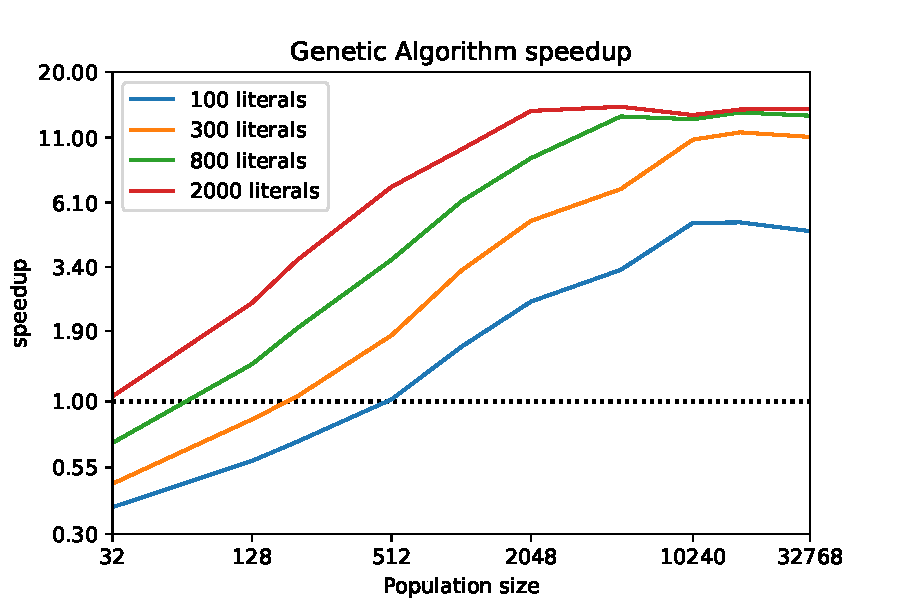
\includegraphics[width=\textwidth]{img/runs/speedup_ga.pdf}
        \caption{Speed up of \acrshort*{acc:ga} on \acrshort*{acc:gpu}}
        \label{fig:gpugaspeedup}
    \end{subfigure}
    \hfill
    \begin{subfigure}[t]{0.45\textwidth}
        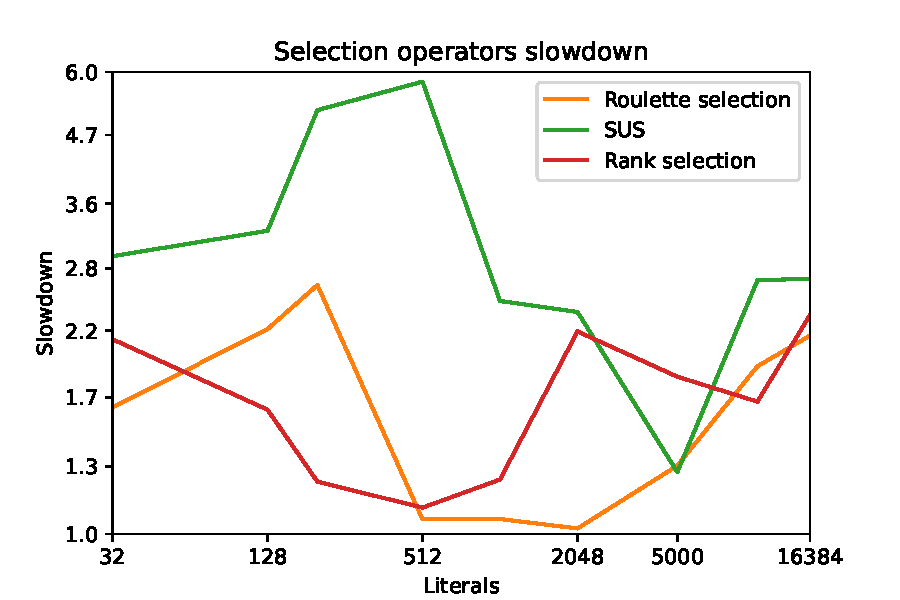
\includegraphics[width=\textwidth]{img/runs/time_ga_selection_slowdown.pdf}
        \caption[Slowdown of GA selection operators]{Slowdown of \acrshort*{acc:ga} on \gpu with various selection operators in constrast to tournament selection}
        \label{fig:gpugaselectionslowdown}
    \end{subfigure}

    \caption{\acrlong*{acc:ga} evaluation}
\end{figure}

The interesting observation is the constant run time of the \gpu implementation for small populations and problems. In these cases, the \gpu is not fully utilized, and the whole population can be processed truly in parallel. As the \cuda cores are less performant than \cpu cores, the total running time is higher than of \cpuns. Moreover, the communication overhead between \cpu and \gpu plays a relevant role in the running time. The speedup of the algorithm running on the \gpu is depicted in figure \ref{fig:gpugaspeedup}.

I compared the PyTorch implementation to \cpp one in figure \ref{meas:cimpl}. You can find the \cpp implementation in the attachment. It used master--worker architecture, where the fitness evaluation is done in parallel using multiple cores, whereas the rest of the algorithm is sequential. Both implementations use the same hyperparameters specified in chapter \ref{chap:hyperparameters}. I compared the implementation using one and eight cores, along with the \gpu implementation. You may notice that \cpp implementation using one core outperforms PyTorch implementation by around $80\%$. Python is an inherently slow language, and the additional overhead of calling native code from Python underlines it. Moreover, the PyTorch implementation is a bit complicated compared to simple \cpp implementation, which may also influence the running time. When I compared the implementations using eight cores, the difference is almost negligible (around $20\%$). The PyTorch implementation took advantage of the parallelization of all the operators, and I believe an increased number of cores would further favor PyTorch implementation. The \gpu implementation still outperforms the \cpp implementation in order of magnitude on populations larger than two thousand individuals.

Of course, one would use a larger population only if it is advantageous. I measured the progress of fitness value over the generation, and these experiments are depicted in figure \ref{meas:gafitness} and \ref{meas:gafitnesselite} (with elitism). I measured the $0.05$ quantile of the fitness function, and the algorithm converges increasingly faster for populations of size $32$, $512$, and $5000$. The big populations with $10240$ and $32768$ individuals do not make an impact until solving big enough \acrshort{acc:3sat} problem with $2000$ and $5000$ literals. Unfortunately, the improvement is not as significant as between the populations of size $512$ and $5000$. In my opinion, using that big population for this kind of problem is not worth it.

Running time of various selection operators in \acrshort{acc:sat} problem is in figure \ref{meas:selection}. Note that this is one of the more noisy experiments, although I repeat the experiment multiple times. For the \cpu implementation, the fitness evaluation is the operator taking most of the time, and the impact of the selection operator is scant. On the \gpu is the situation different, and the selection operators seem to have an order of magnitude difference. The fastest one is the tournament selection, which is not surprising, as it does not require sorting or search in the fitness array in any way. On the other hand, the \acrshort{acc:sus} seems to be the slowest of them, especially for smaller populations. For bigger populations of the size greater than $5000$ the performance of roulette, \acrshort{acc:sus} and rank selection look very similar. You can see the slowdown of these operators in comparison to tournament selection in figure \ref{fig:gpugaselectionslowdown}. As you may notice, the measurements are unfortunately very noisy.

Lastly, I measured the impact of fitness scaling operators on the run time of the \acrshort{acc:ga}, and these results are in figure \ref{meas:scale}. The algorithm used tournament selection, and the different scale operators did not influence the algorithm's performance. Similarly to the selection, the fitness evaluation took the longest time, and the execution of the scale function does not make any impact when executed on \cpu (including the rank scale operator). The situation with \gpu was very similar except for a small problem ($100$ literals and $450$ clauses), where logarithmic, exponential, and rank scaling took slightly more time.

I tested mutation operators on real--coded evolutionary algorithm with uniform crossover and tournament selection; the results are in figure \ref{meas:muttime} and their fitness in figure \ref{meas:mutfitness}. Both \cpu and \gpu implementation were slowest using Cauchy mutation. This reason is that the sampling from the Cauchy distribution lacks efficient implementation. The fastest was normal mutation with replacement mutation in some \gpu cases (on \cpu the replacement mutation was always a bit slower than the normal mutation). The adaptive step mutation was somewhere in between because of the extra overhead of comparing new fitness values to the old ones. The replacement mutation is interesting, as it outperformed normal mutation on some cases on \gpuns but is steadily slower on \cpuns. I believe sampling random value within an interval would be faster than sampling from the normal distribution, and I cannot fully explain this.

From a convergence point of view, the experiments are shown in figure \ref{meas:mutfitness}. The best performant mutation is the normal mutation, and as it is the fastest one, I would recommend it. Unfortunately, the various mutation operators do not take advantage of a bigger population, and except for population size $32$, the performance of populations with sizes $10240$ and $32768$ is the same. The algorithm converged a little faster with $10240$ individuals instead of $512$, but only for a problem with $384$ dimensions, and the difference is negligible. The only exception worth mentioning is the normal and Cauchy mutation for a problem with $24$ dimensions, where a larger population helped find better optima. Lastly, you may notice better convergence properties of adaptive step mutation in contrast to normal or Cauchy mutation.

The crossover operators were tested on real--coded evolutionary algorithm, and the running times are in figure \ref{meas:crosstime} along with their fitness values in figure \ref{meas:crossfitness}. The running times were of the same order for all of them. The slowest on the \cpu was the blend crossover, while the arithmetic crossover was the fastest one. The slowest on the \cpu was the two--points crossover because of the complicated creation of the mask, as discussed in the chapter \ref{chap:impl}. The fastest operator for small populations was the arithmetic crossover with the blend crossover. The running time for big populations on \gpu was almost identical for all the operators. Unlike mutation operators, some of the crossover operators take advantage of the larger population, as shown in figure \ref{meas:crossfitness} -- for example the one--point and two--point crossovers. On the other hand, blend crossover performed best using $512$ individuals, and a bigger population decreased its performance.

Lastly, the crossover schema experiments are depicted in figure \ref{meas:schema}. There is no surprise that the default schema (that is, the offsprings replace their parents in the population) is the fastest one because it does not require extra memory allocation, as discussed in section \ref{chap:gaimpl}. It is followed by comma schema, which is almost two times slower. The plus schema is the slowest and runs around $2.3\times$ slower than the default schema.

Finally, the running time of \acrshort{acc:spso2006} and \acrshort{acc:spso2011} algorithms are shown in the figure \ref{meas:spso2006time} and \ref{meas:spso2011time}. The \acrshort{acc:pso} algorithms show bigger speedup than \acrshort{acc:ga} and real--coded evolutionary algorithms, even for problems with $384$ dimensions. The running times for problem with $6$, $32$, and $128$ dimensions is almost identical except the \acrshort{acc:bbob} function $f_{22}$. This function has the most complicated evaluation and takes great portion of the running time. The graphs showing average fitness are in figures \ref{meas:spso2006fitness} (for \acrshort{acc:spso2006}) and \ref{meas:spso2011fitness} (for \acrshort{acc:spso2011}). Unlike in previous experiments, all the problems take advantage of the larger population, as is clearly visible in the figures. I would say the \acrshort{acc:pso} algorithms has the biggest potential to run on \gpuns.

The \acrshort{acc:pso} neighborhoods experiments are depicted in figure \ref{meas:psoneigtime}, and their fitness in figure \ref{meas:psoneigfitness}. The random and circle neighborhoods are the fastest to evaluate on \gpuns, where the circle one is a bit faster for small populations. The circle neighborhood is static and generated only once, while the random neighborhood changes with every iteration. On the other hand, the random neighborhood is the slowest on the \cpu (except the nearest one). The grid--based neighborhoods are as fast as circle neighborhood for smaller populations, but for bigger populations the evaluation takes as long as random neighborhood. The cause is their substantial size in contrast to the circle one. The nearest neighborhood is extensively slower than any other. This is expected because it needs to measure the distance between every pair of particles, which is very costly even on \gpuns. The neighborhood evaluation is still more than six times faster on the \gpu than on the \cpu for swarms larger than $500$ particles.
\chapter{Conclusion}
\label{chap:conclusion}

This work summarizes current knowledge of \acrlong*{acc:ea} and gives a comprehensive overview of this research field. It discusses the well--known evolutionary operators and gives their detailed analysis from the implementation point of view, along with their desired properties. The work further describes the three most common evolutionary algorithms -- the \acrlong{acc:ga}, real--\kern0.04em coded evolutionary algorithms, and the \acrlong{acc:pso} algorithms. Each of them is analyzed, and their representative operators are described and examined.

The work further discusses the differences between \cpu and \gpu and their architectures. I show that while the \gpu has its application in various fields mentioned in the work, the mindset for programming on \gpu is considerably different and unique. I present the OpenCL and \cuda technologies, and present the terminology used in \gpu programming. The work shows the elements of \cuda programming, with a particular focus on a performance issue that can arise. 

I then present the PyTorch library for the Python programming language, describe its architecture and functionality. The work put into connection the PyTorch library and \cuda programming discussed before. Follows discussion about possible ways to parallelize \acrlong{acc:ea} both on \cpu and \gpuns. The work focuses on different individual encoding, parallelization granularity, and evaluation architectures.

Follows presentation of the \acrfull{acc:ffeat}, my contribution to this area. I discuss in detail its functionality, implementation decisions, architecture, and the proposed workflow. The work gives extra space to challenging parts of the implementation, like parental sampling and crossover schemes. Some of these problems arise from the limitations of the PyTorch library and the \cuda programming in general; these aspects are discussed. Implementation of some operators is then shown in the text, and I discuss possible ways to extend the library. Overall, I show that the proposed implementation is easy to extend, operators are written in a readable manner and runs efficiently on \gpuns.

The implementation is subjected to extensive testing on \acrshort{acc:3sat} problem and \acrshort{acc:bbob} test suite. The experiments show the advantage of using \cuda implementation for medium and big--sized populations and problems. The experiments show an order of magnitude speedup using \cuda implementation rather than \cpuns. Moreover, the experiments show the advantage of a bigger population on some problems while leading to premature convergence on others. I discuss this phenomenon and explain the behavior of algorithms.

Finally, I compare the proposed implementation against the native \cpp implementation on the \acrshort{acc:3sat} problem. It shows a noticeable slowdown on one core machine but gets faster as the number of cores increases. The proposed implementation makes use of the parallelized operators implementation and becomes dominant. The comparison with \cpp implementation confirms the superiority of \cuda implementation for medium and big--sized populations.

This work dealt with \acrshort{acc:ga}, real--\kern0.04em coded evolutionary algorithms, and \acrshort{acc:pso} algorithms. There are other classes of algorithms that the implementation was not tested on. Further work could expand the library with these algorithms. I believe the \acrshort{acc:cma} would greatly benefit of \cuda implementation. Benchmark the implementation on permutation--based algorithms may seems interesting as well. Furthermore, all the presented problems have been vectorized, and the \gpu implementation could evaluate the whole population at once. It may be interesting to explore the possibility of evaluating each individual separately, taking away the major advantage of \gpu implementation. This may be practical for complicated fitness functions. Future work could explore this possibility and evaluate whether using \gpu implementation keeps its advantages.

%%% Bibliography
%%% Bibliography (literature used as a source)
%%%
%%% We employ bibTeX to construct the bibliography. It processes
%%% citations in the text (e.g., the \cite{...} macro) and looks up
%%% relevant entries in the bibliography.bib file.
%%%
%%% The \bibliographystyle command selects, which style will be used
%%% for references from the text. The argument in curly brackets is
%%% the name of the corresponding style file (*.bst). Both styles
%%% mentioned in this template are included in LaTeX distributions.

%\bibliographystyle{plainnat}   %% Author (year)
%\bibliographystyle{unsrt}      %% [number]
\bibliographystyle{apalike}    %% [Author, year]      

%\renewcommand{\bibname}{Bibliography}

%%% Generate the bibliography. Beware that if you cited no works,
%%% the empty list will be omitted completely.
\bibliography{bibliography,bibliographyintro}


%%% Figures used in the thesis (consider if this is needed)
\listoffigures

%%% Tables used in the thesis (consider if this is needed)
%%% In mathematical theses, it could be better to move the list of tables to the beginning of the thesis.
\listoftables

\listofalgorithms

%%% Abbreviations used in the thesis, if any, including their explanation
%%% In mathematical theses, it could be better to move the list of abbreviations to the beginning of the thesis.
%\chapwithtoc{List of Abbreviations}
\printglossary
\printglossary[type=\acronymtype, nonumberlist,title={List of Abbreviations}]

%%% Attachments to the master thesis, if any. Each attachment must be
%%% referred to at least once from the text of the thesis. Attachments
%%% are numbered.
%%%
%%% The printed version should preferably contain attachments, which can be
%%% read (additional tables and charts, supplementary text, examples of
%%% program output, etc.). The electronic version is more suited for attachments
%%% which will likely be used in an electronic form rather than read (program
%%% source code, data files, interactive charts, etc.). Electronic attachments
%%% should be uploaded to SIS and optionally also included in the thesis on a~CD/DVD.
%%% Allowed file formats are specified in provision of the rector no. 72/2017.
\appendix

\printindex
% TODO přidat vše do indexu

\chapter{Selected Operators Implementation}
\label{chap:examples}

\begin{algorithm}
\begin{lstlisting}[language=Python, xrightmargin=18pt, breaklines=true, postbreak=\mbox{$\hookrightarrow$\space}, literate={\ \ }{{\ }}1]
from typing import Tuple, Any, Dict, Union, Callable
import torch as t
from ffeat import Pipe
from ffeat.utils._parental_sampling import randint

_IFU = Union[int, float]

class Tournament(Pipe):
    def __init__(self, num_select=None, maximization=False, parents=2, parental_sampling=randint):
        self._num_select = self._handle_parameter(num_select)
        self._maximization=maximization
        self._parents = parents
        self._parental_sampling = parental_sampling

    def __call__(self, fitnesses, population, *args, **kwargs):
        originally = len(population)
        to_select = self._num_select(fitnesses, population, *args, **kwargs)

        indices = self._parental_sampling(originally, to_select, self._parents, fitnesses.device)
        operation = t.argmax if self._maximization else t.argmin
        best_indices = operation(fitnesses[indices], dim=1)
        selected = population[indices[range(to_select),best_indices]]

        return (selected, *args), kwargs
\end{lstlisting}
\caption{Tournament selection implementation}
\label{alg:impltournament}
\end{algorithm}

\begin{algorithm}
\begin{lstlisting}[language=Python, xrightmargin=18pt, breaklines=true, postbreak=\mbox{$\hookrightarrow$\space}, literate={\ \ }{{\ }}1]
from typing import Tuple, Any, Dict, Union
import torch as t
from ffeat import Pipe
from ._Shared import _CommonCrossover
from ffeat.utils._parental_sampling import randint

class OnePoint1D(Pipe, _CommonCrossover):
    def __init__(self, offsprings, replace_parents=True, in_place=True, discard_parents=False, parental_sampling=randint):
        _Shared.__init__(self, offsprings, replace_parents, in_place, discard_parents)
        self._parental_sampling = parental_sampling

    def __call__(self, population, *args, **kwargs):
        ptp = population.dtype if population.dtype != t.bool else t.uint8
        dev = population.device
        dim = population.shape[1]
        num_crossovers = self._offsprings // 2
        crossover_indices = t.randint(1, dim, size=(num_crossovers,), dtype=t.long, device=dev)
        parents_indices = self._parental_sampling(len(population), num_crossovers, 2, dev).T
        children = t.zeros((num_crossovers, dim), dtype=ptp, device=dev)
        position_mask = t.arange(dim, device=dev).as_strided((num_crossovers,dim), (0,1))
        lpos = (position_mask < crossover_indices[:, None]).type(t.int8)
        children[:num_crossovers].add_(population[parents_indices[0]] * lpos)
        children[num_crossovers:].add_(population[parents_indices[1]] * lpos)
        rpos = t.logical_not(lpos, out=lpos)
        children[:num_crossovers].add_(population[parents_indices[1]] * rpos)
        children[num_crossovers:].add_(population[parents_indices[0]] * lpos)
        children = children.to(population.dtype)
        pop = self._handle_pop(population, children, parents_indices)
        return (pop, *args), kwargs
\end{lstlisting}
\caption{One--point crossover operator}
\label{alg:implonepoint}
\end{algorithm}

\begin{algorithm}
\begin{lstlisting}[language=Python, xrightmargin=18pt, breaklines=true, postbreak=\mbox{$\hookrightarrow$\space}, literate={\ \ }{{\ }}1]
from typing import Tuple, Any, Dict, Union, Callable
import torch as t
from ffeat import Pipe, flow

class Elitism(Pipe):
    def __init__(self,
                 num_elites,
                 *following_steps,
                 maximization=False):
        self._num_elites = self._handle_parameter(num_elites)
        self._maximization = maximization
        self.__follow = flow.Sequence(*following_steps)

    def __call__(self, fitnesses, population, *args, **kwargs):
        to_select = self._num_elites(fitnesses, population, *args, **kwargs)
        elites_indices = t.topk(fitnesses, to_select, largest=self._maximization)[1]
        elites = t.clone(population[elites_indices])
        (population, *args), kargs = self.__follow(fitnesses, population, *args, **kwargs)
        population[elites_indices] = elites
        return (population, *args), kwargs
\end{lstlisting}
\caption{Elitism operator implementation}
\label{alg:implelitism}
\end{algorithm}
\chapter{Hyperparameters}

\begin{table}[h]
    \centering
    \begin{tabular}{|l r|c|}
        \hline
        \multicolumn{2}{|c|}{\textbf{Parameter}} & \thead{Value} \\
        \hline
        cognitive acceleration coefficient & $c_l$ & 1.5 \\
        social acceleration coefficient  & $c_g$ & 1.5 \\
        inertia weight & $\omega$ & 0.8 \\
        velocity clip value & & 2 \\
        \hline \hline
        \textbf{Neighborhood} & & \makecell[c]{Size in\\ percent} \\
        \hline
        Circle & & 0.26 \\
        Grid & & \\
        \quad linear & & 0.02 \\
        \quad compact & & 0.05 \\
        \quad diamond & & 0.06 \\
        Nearest neighbors & & 0.13 \\
        Random & & \\
        \quad PSO2006 & & 0.13 \\
        \quad PSO2011 & & 0.2 \\ 
        \hline
    \end{tabular}
    \caption{\acrlong*{acc:pso} hyperparameters}
\end{table}
\chapter{Results}

All the algorithms were run with hyperparameters from chpater \ref{chap:hyperparameters}. Each configuration run a hundred times and the plotted values are mean of specified metric.



%%%%%%%%%%%%%%%%%
%%             %%
%%   GENETIC   %%
%%             %%
%%%%%%%%%%%%%%%%%
\begin{figure}[ht!]
    \centering
    \begin{minipage}[t]{0.5\textwidth}
        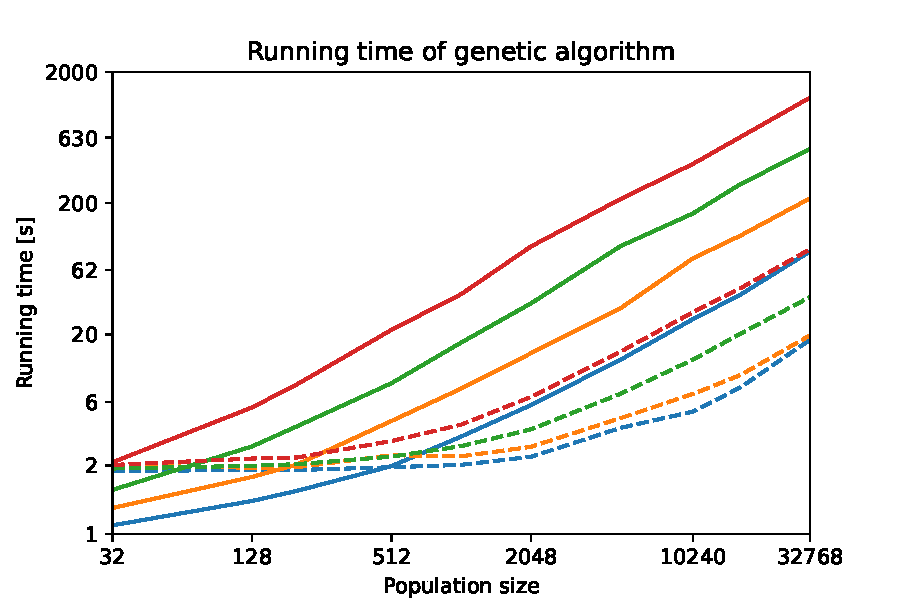
\includegraphics[width=\textwidth]{img/runs/time_ga.pdf}
    \end{minipage}

    \begin{minipage}{0.6\textwidth}
        \centering
        
\includegraphics[width=\textwidth]{img/runs/time_ga_legend.pdf}
    \end{minipage}

    \caption[Running times of genetic algorithm]{Genetic algorithm running time. \todo{Dopsat popisek.}}
\end{figure}




%%%%%%%%%%%%%%%%%%%%%%
%%                  %%
%%   ES MUTATIONS   %%
%%                  %%
%%%%%%%%%%%%%%%%%%%%%%
\begin{figure}[ht!]
    \begin{minipage}[t]{0.32\textwidth}
        \centering
        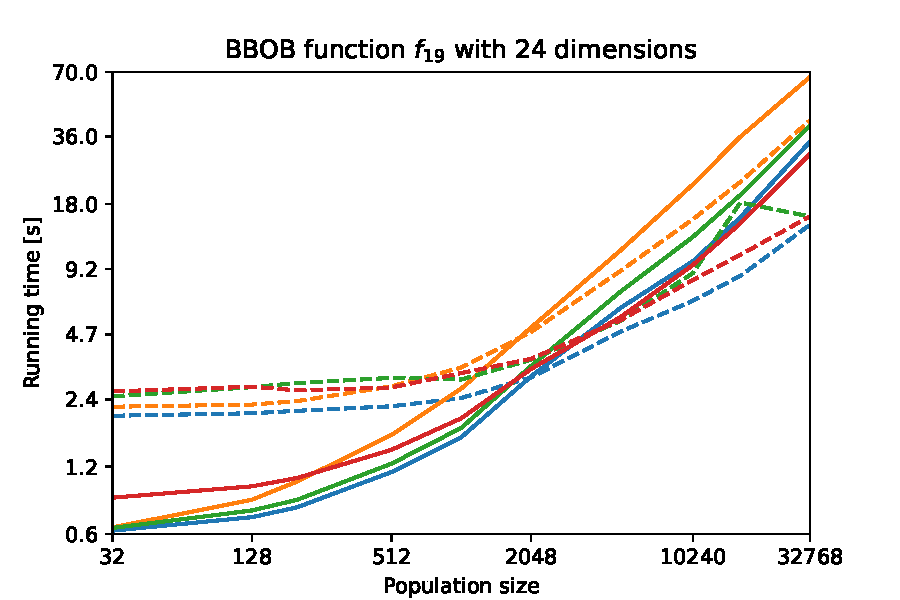
\includegraphics[width=\textwidth]{img/runs/time_es_mutation_fn19_24d.pdf}
    \end{minipage}
    \hfill
    \begin{minipage}[t]{0.32\textwidth}
        \centering
        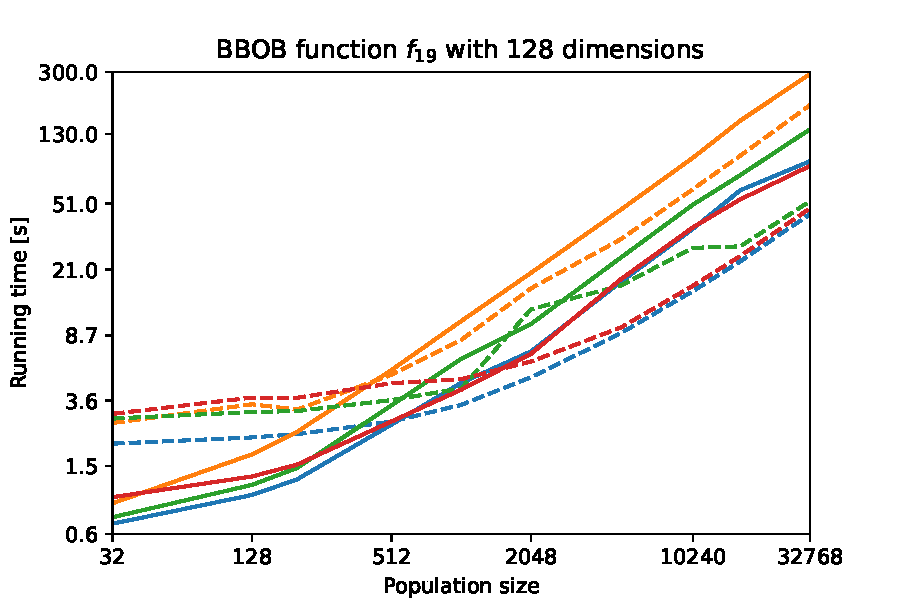
\includegraphics[width=\textwidth]{img/runs/time_es_mutation_fn19_128d.pdf}
    \end{minipage}
    \hfill
    \begin{minipage}[t]{0.32\textwidth}
        \centering
        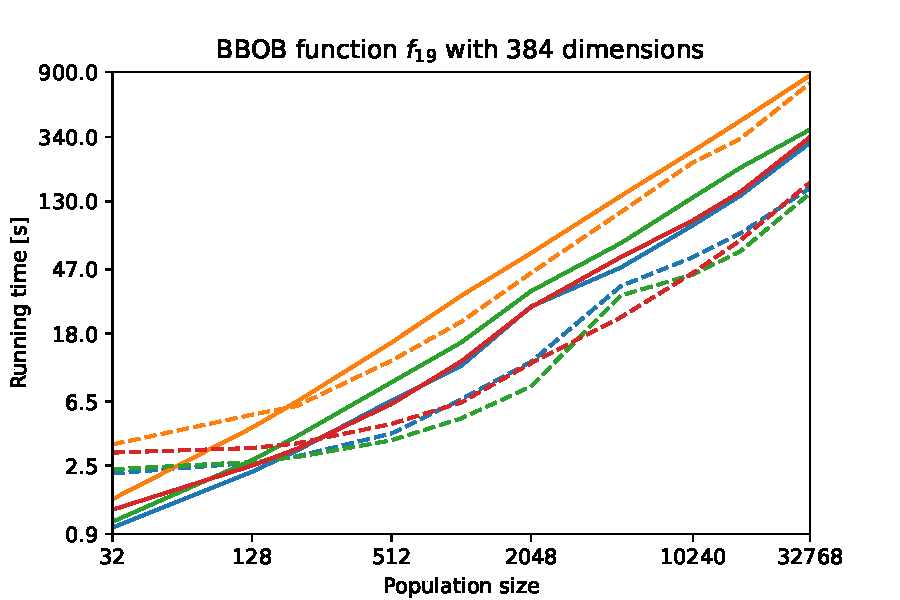
\includegraphics[width=\textwidth]{img/runs/time_es_mutation_fn19_384d.pdf}
    \end{minipage}

    \begin{minipage}[t]{0.32\textwidth}
        \centering
        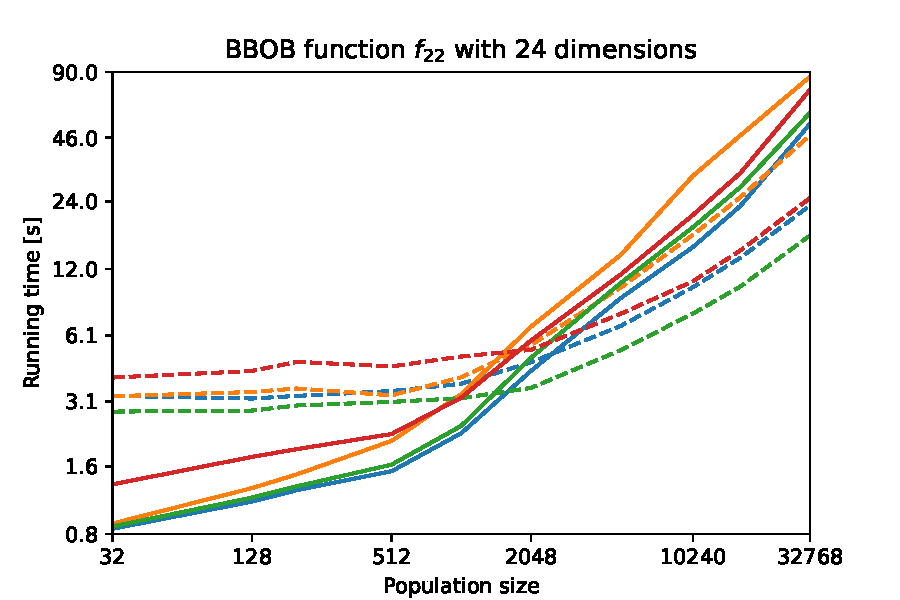
\includegraphics[width=\textwidth]{img/runs/time_es_mutation_fn22_24d.pdf}
    \end{minipage}
    \hfill
    \begin{minipage}[t]{0.32\textwidth}
        \centering
        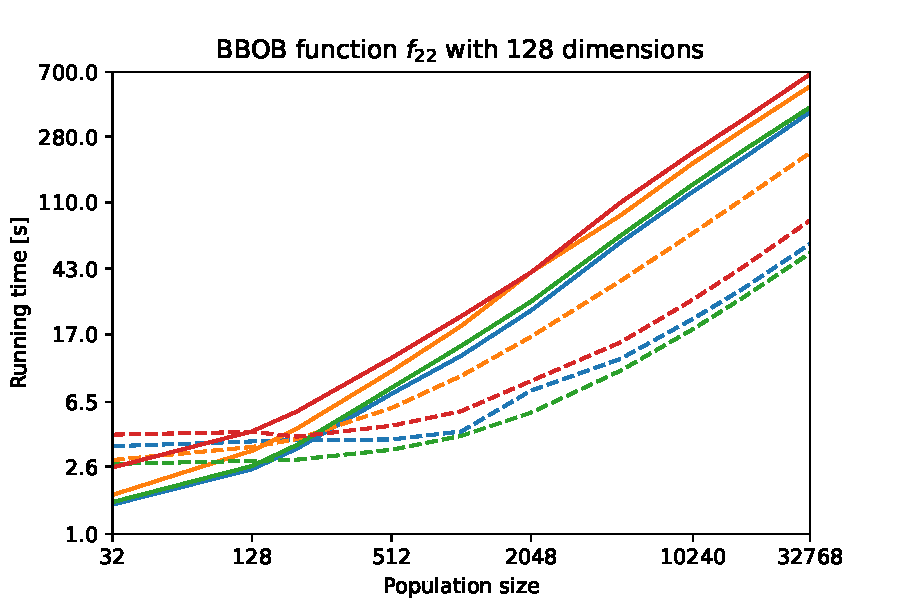
\includegraphics[width=\textwidth]{img/runs/time_es_mutation_fn22_128d.pdf}
    \end{minipage}
    \hfill
    \begin{minipage}[t]{0.32\textwidth}
        \centering
        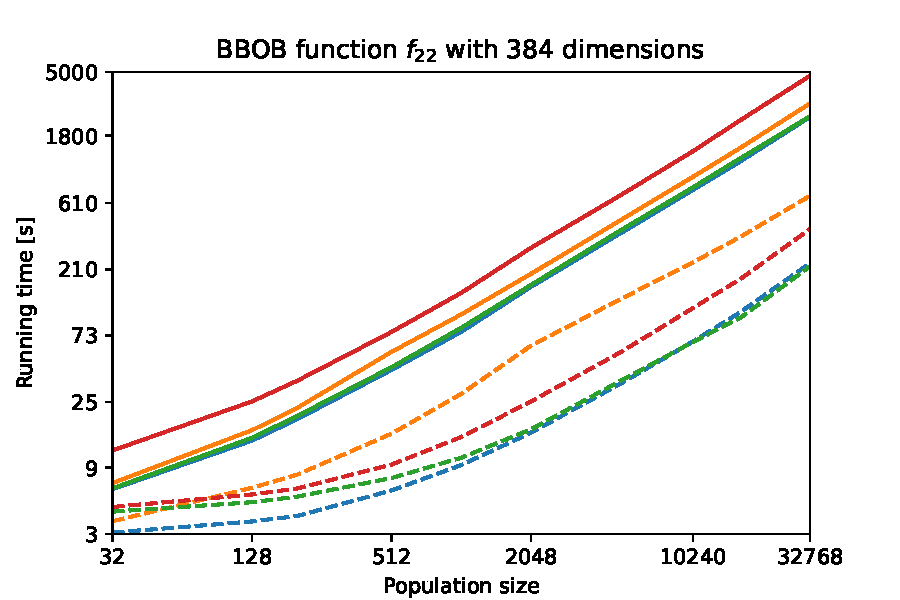
\includegraphics[width=\textwidth]{img/runs/time_es_mutation_fn22_384d.pdf}
    \end{minipage}

    \begin{minipage}{\textwidth}
        \centering
        
\includegraphics[width=0.8\textwidth]{img/runs/time_es_mutation_legend.pdf}
    \end{minipage}

    \caption[Running times of mutation operators]{Running times of various mutation operators for real--coded evolutionary algorithms. I chose to measure only \acrshort{acc:bbob} functions $f_{19}$ and $f_{22}$. \todo{Dopsat popisek.}}
\end{figure}



\begin{figure}[ht!]
    \begin{minipage}[t]{0.32\textwidth}
        \centering
        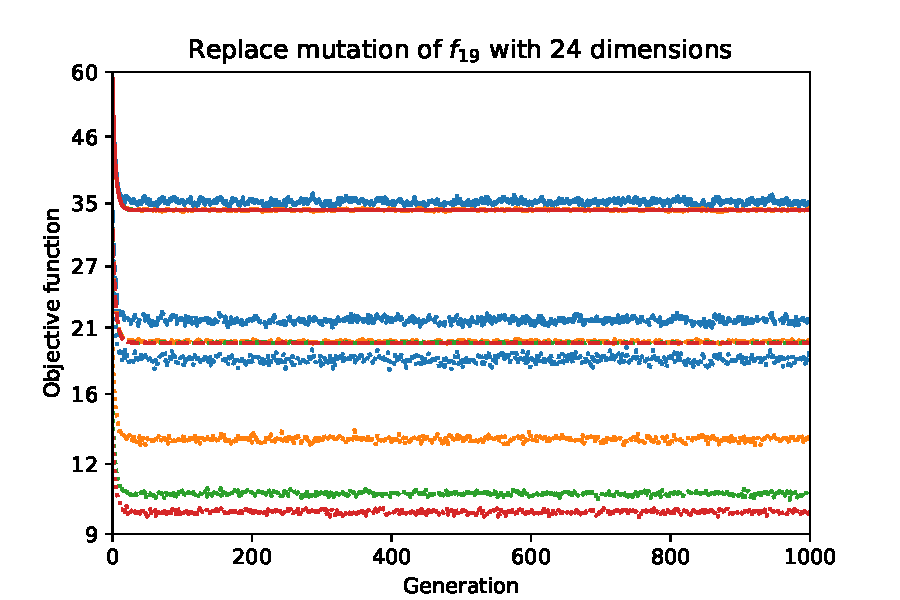
\includegraphics[width=\textwidth]{img/runs/fitness_es_mutation_f19_dim24_ReplaceUniform.pdf}
    \end{minipage}
    \hfill
    \begin{minipage}[t]{0.32\textwidth}
        \centering
        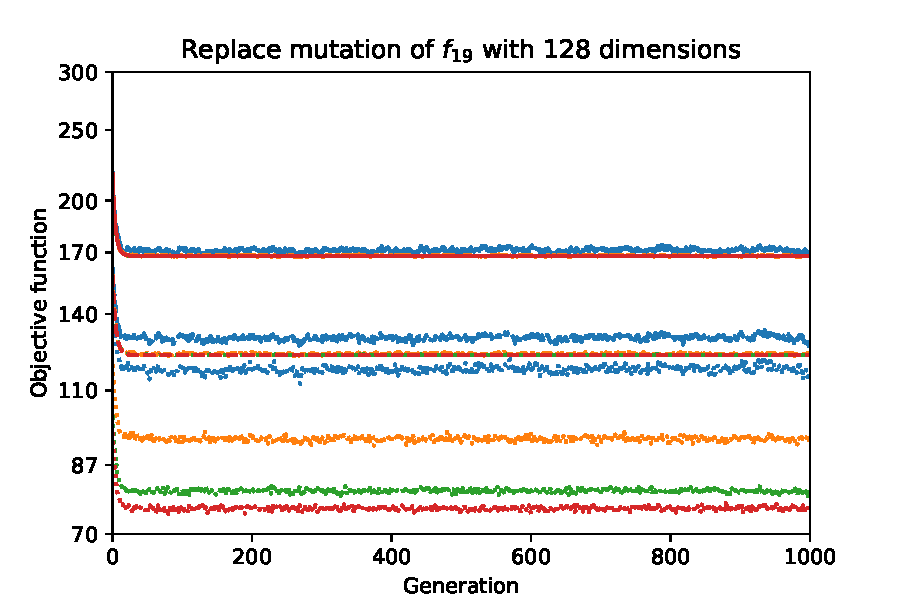
\includegraphics[width=\textwidth]{img/runs/fitness_es_mutation_f19_dim128_ReplaceUniform.pdf}
    \end{minipage}
    \hfill
    \begin{minipage}[t]{0.32\textwidth}
        \centering
        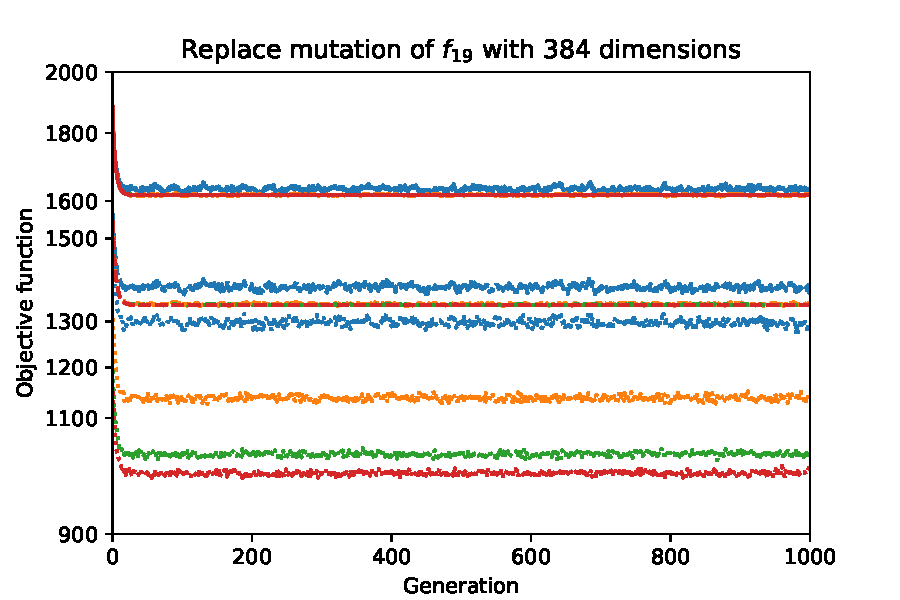
\includegraphics[width=\textwidth]{img/runs/fitness_es_mutation_f19_dim384_ReplaceUniform.pdf}
    \end{minipage}

    \begin{minipage}[t]{0.32\textwidth}
        \centering
        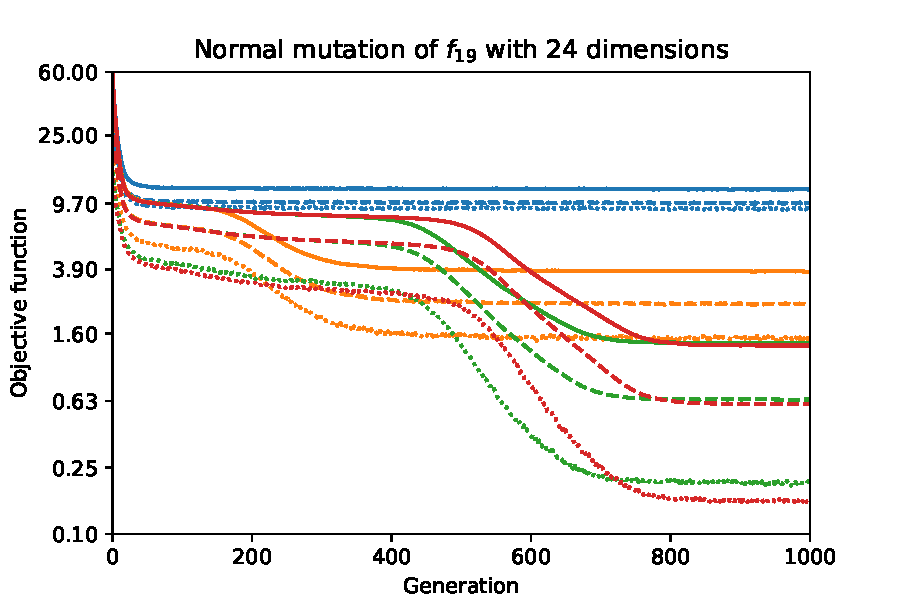
\includegraphics[width=\textwidth]{img/runs/fitness_es_mutation_f19_dim24_AddFromNormal.pdf}
    \end{minipage}
    \hfill
    \begin{minipage}[t]{0.32\textwidth}
        \centering
        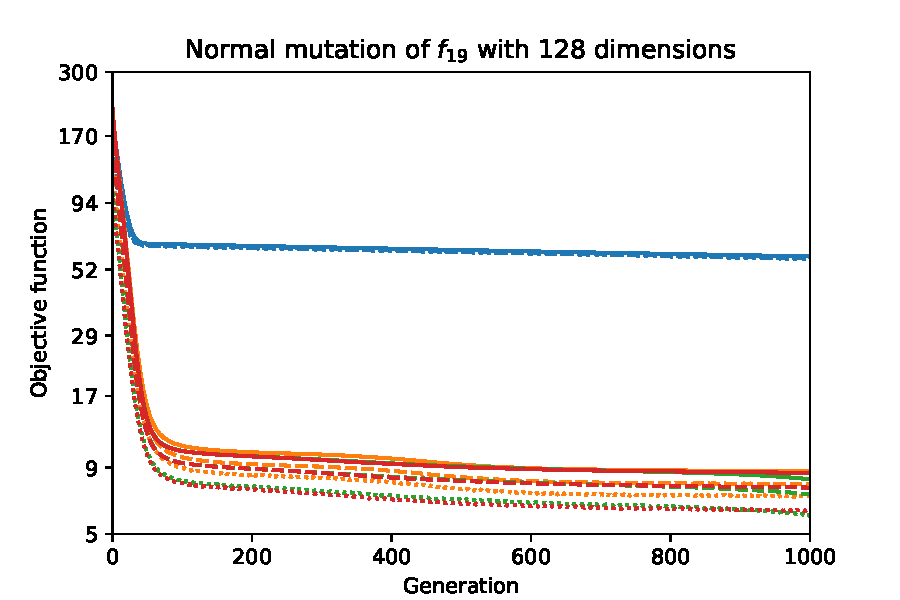
\includegraphics[width=\textwidth]{img/runs/fitness_es_mutation_f19_dim128_AddFromNormal.pdf}
    \end{minipage}
    \hfill
    \begin{minipage}[t]{0.32\textwidth}
        \centering
        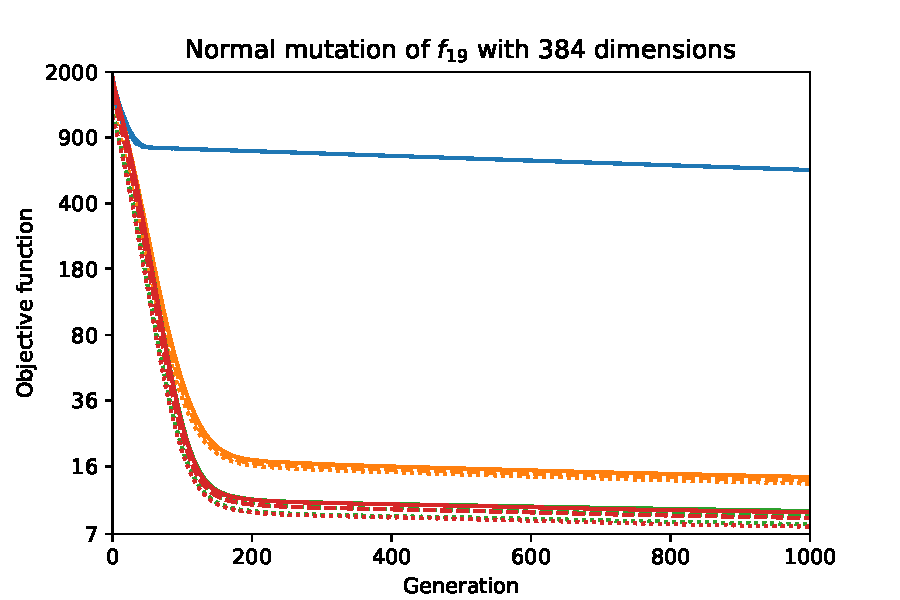
\includegraphics[width=\textwidth]{img/runs/fitness_es_mutation_f19_dim384_AddFromNormal.pdf}
    \end{minipage}

    \begin{minipage}[t]{0.32\textwidth}
        \centering
        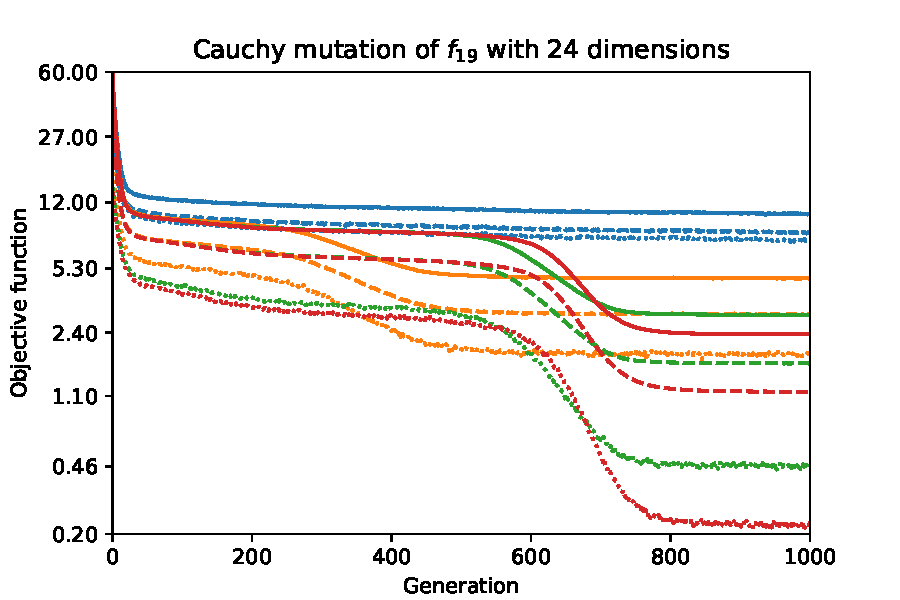
\includegraphics[width=\textwidth]{img/runs/fitness_es_mutation_f19_dim24_AddFromCauchy.pdf}
    \end{minipage}
    \hfill
    \begin{minipage}[t]{0.32\textwidth}
        \centering
        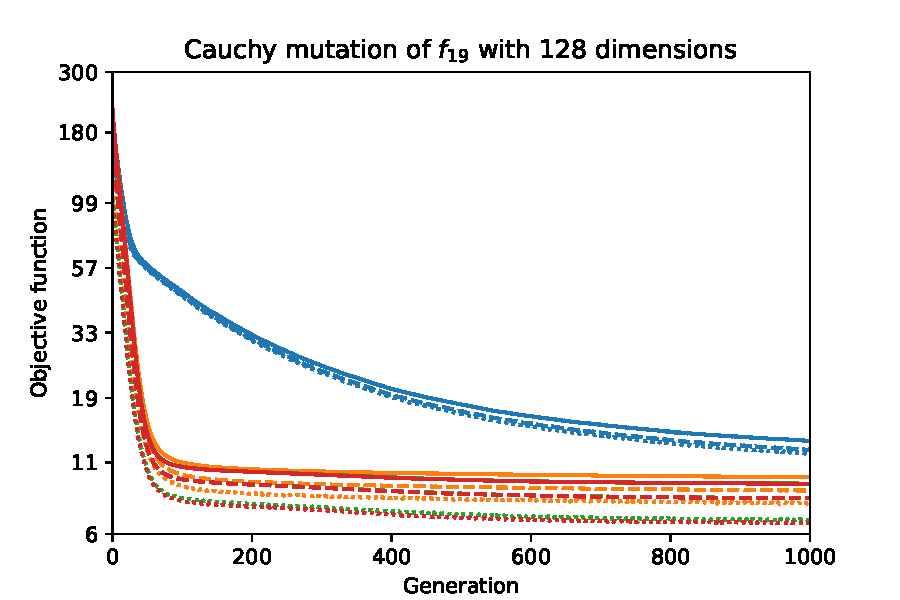
\includegraphics[width=\textwidth]{img/runs/fitness_es_mutation_f19_dim128_AddFromCauchy.pdf}
    \end{minipage}
    \hfill
    \begin{minipage}[t]{0.32\textwidth}
        \centering
        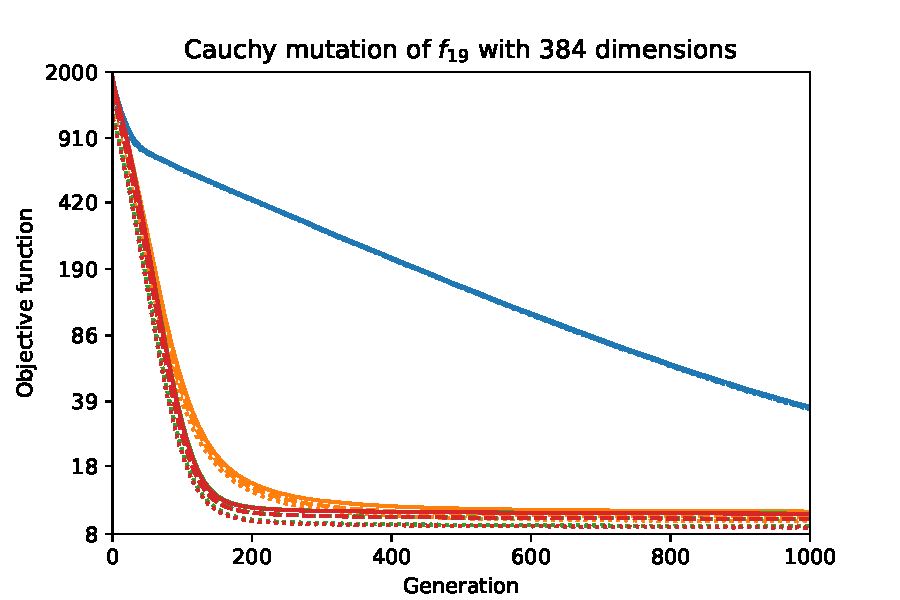
\includegraphics[width=\textwidth]{img/runs/fitness_es_mutation_f19_dim384_AddFromCauchy.pdf}
    \end{minipage}

    \begin{minipage}[t]{0.32\textwidth}
        \centering
        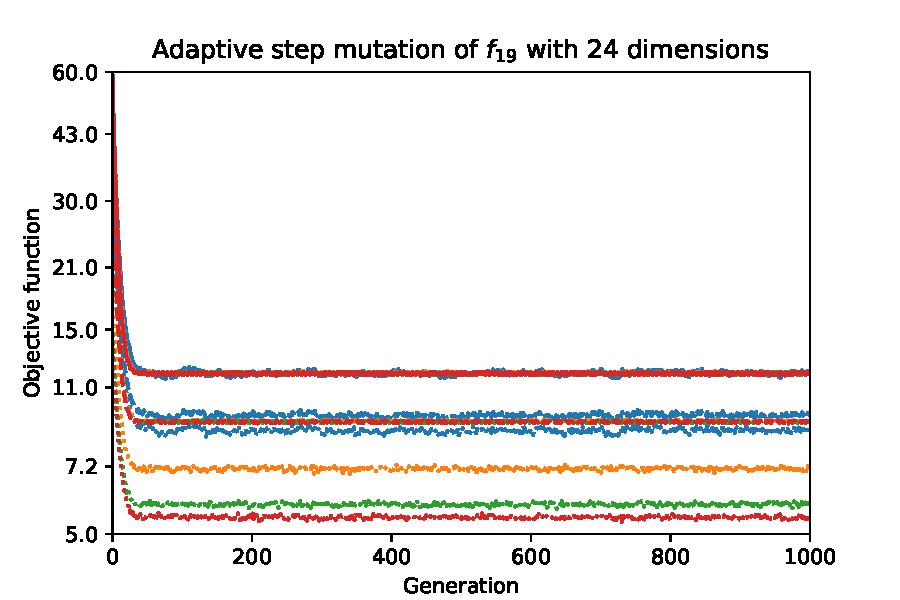
\includegraphics[width=\textwidth]{img/runs/fitness_es_mutation_f19_dim24_AdaptiveStep.pdf}
    \end{minipage}
    \hfill
    \begin{minipage}[t]{0.32\textwidth}
        \centering
        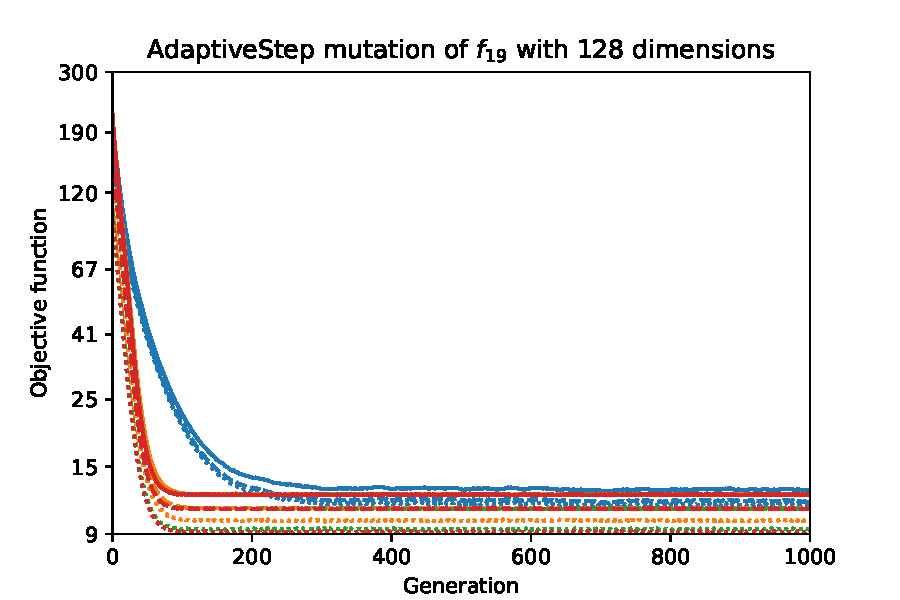
\includegraphics[width=\textwidth]{img/runs/fitness_es_mutation_f19_dim128_AdaptiveStep.pdf}
    \end{minipage}
    \hfill
    \begin{minipage}[t]{0.32\textwidth}
        \centering
        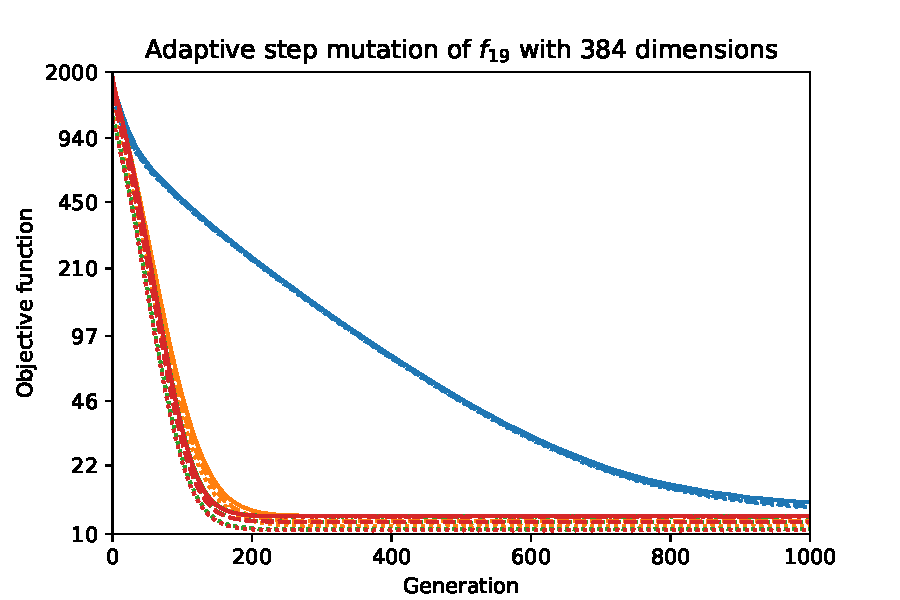
\includegraphics[width=\textwidth]{img/runs/fitness_es_mutation_f19_dim384_AdaptiveStep.pdf}
    \end{minipage}

    \begin{minipage}{\textwidth}
        \centering
        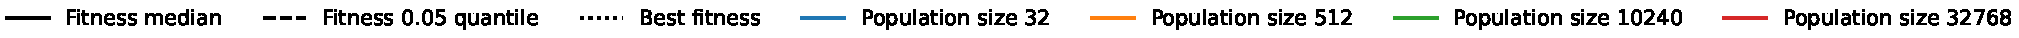
\includegraphics[width=\textwidth]{img/runs/fitness_es_mutation_legend.pdf}
    \end{minipage}

    \caption[Real--coded mutation fitness over generations]{\todo{Real--coded mutation fitness over generations. Dopsat zbytek.}}
\end{figure}



%%%%%%%%%%%%%%%%%%%%%%%
%%                   %%
%%   ES CROSSOVERS   %%
%%                   %%
%5%%%%%%%%%%%%%%%%%%%%%
\begin{figure}[ht!]
    \begin{minipage}[t]{0.32\textwidth}
        \centering
        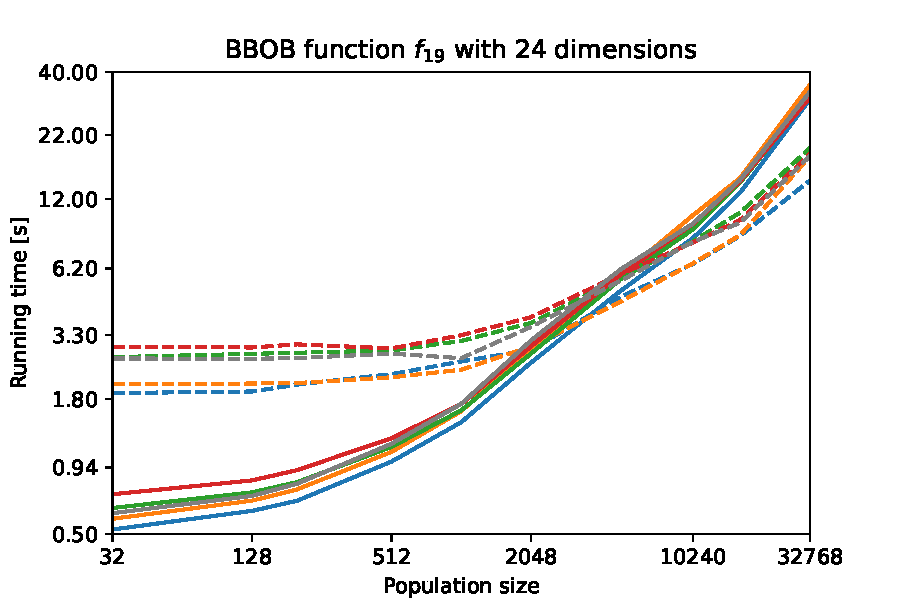
\includegraphics[width=\textwidth]{img/runs/time_es_crossover_fn19_24d.pdf}
    \end{minipage}
    \hfill
    \begin{minipage}[t]{0.32\textwidth}
        \centering
        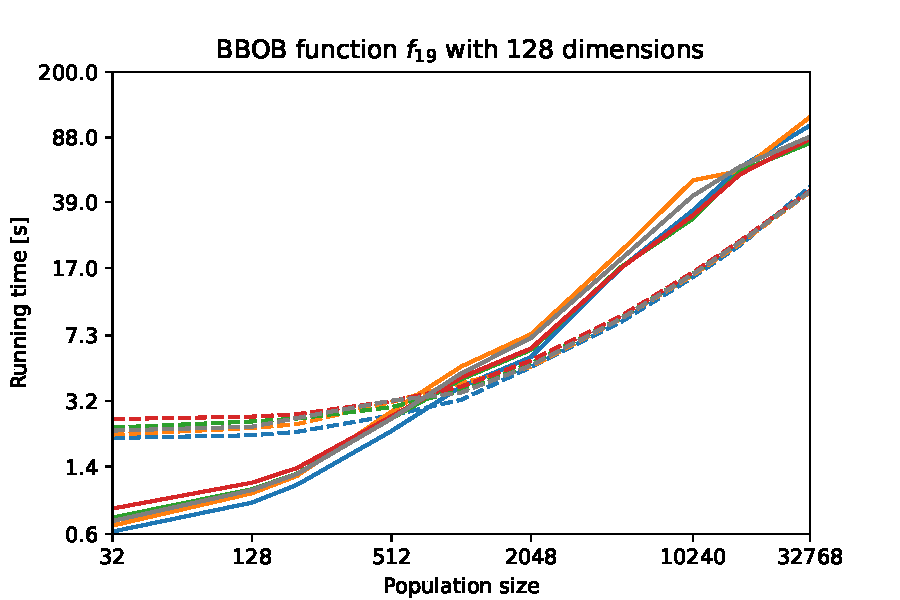
\includegraphics[width=\textwidth]{img/runs/time_es_crossover_fn19_128d.pdf}
    \end{minipage}
    \hfill
    \begin{minipage}[t]{0.32\textwidth}
        \centering
        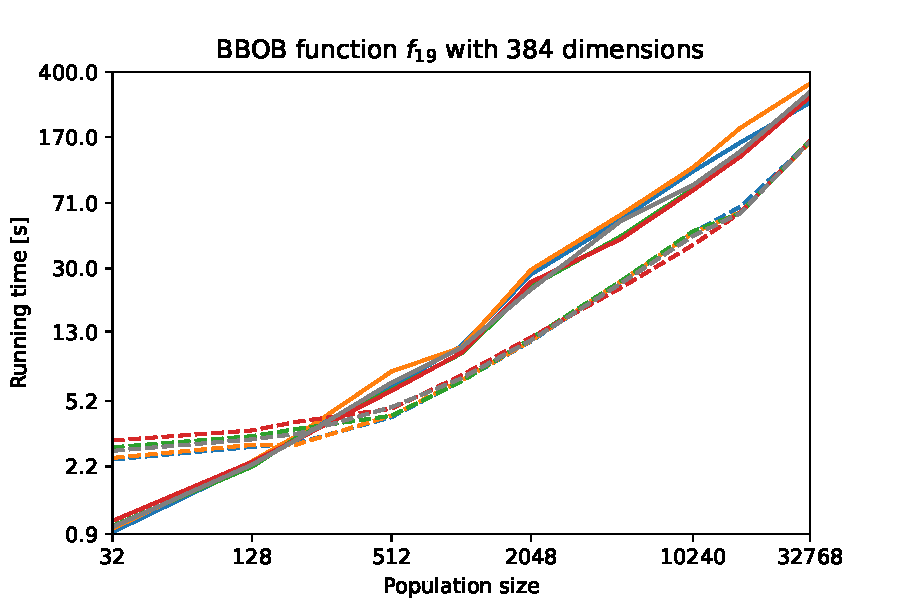
\includegraphics[width=\textwidth]{img/runs/time_es_crossover_fn19_384d.pdf}
    \end{minipage}

    \begin{minipage}[t]{0.32\textwidth}
        \centering
        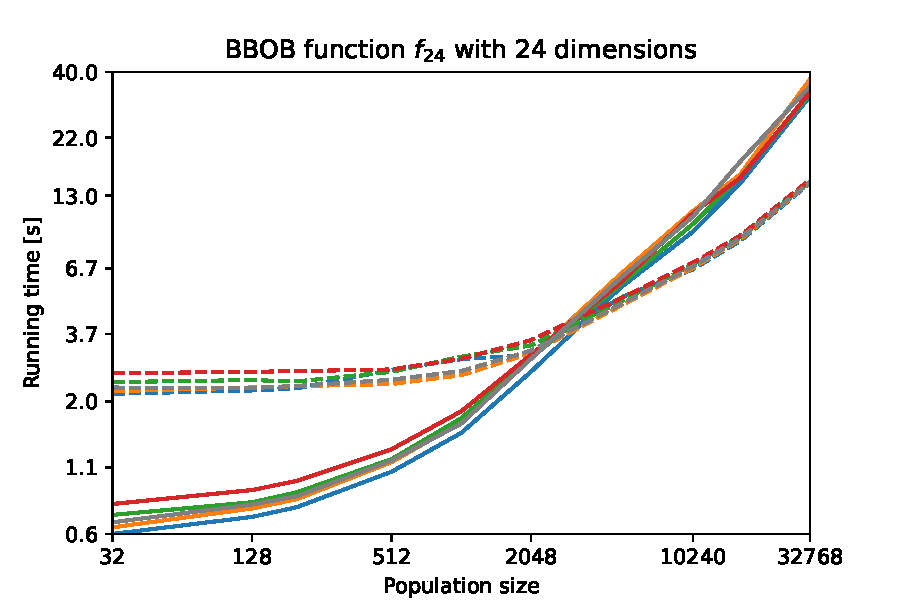
\includegraphics[width=\textwidth]{img/runs/time_es_crossover_fn24_24d.pdf}
    \end{minipage}
    \hfill
    \begin{minipage}[t]{0.32\textwidth}
        \centering
        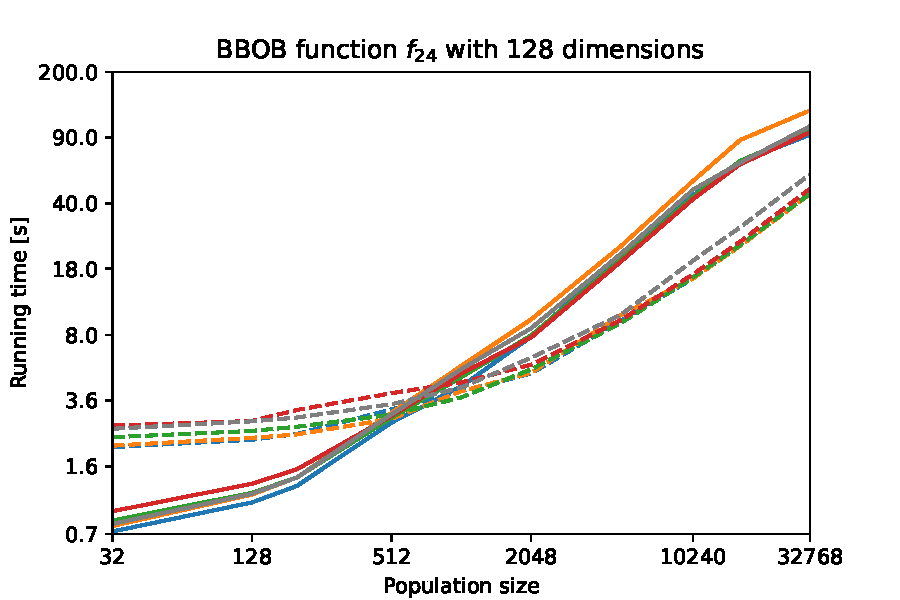
\includegraphics[width=\textwidth]{img/runs/time_es_crossover_fn24_128d.pdf}
    \end{minipage}
    \hfill
    \begin{minipage}[t]{0.32\textwidth}
        \centering
        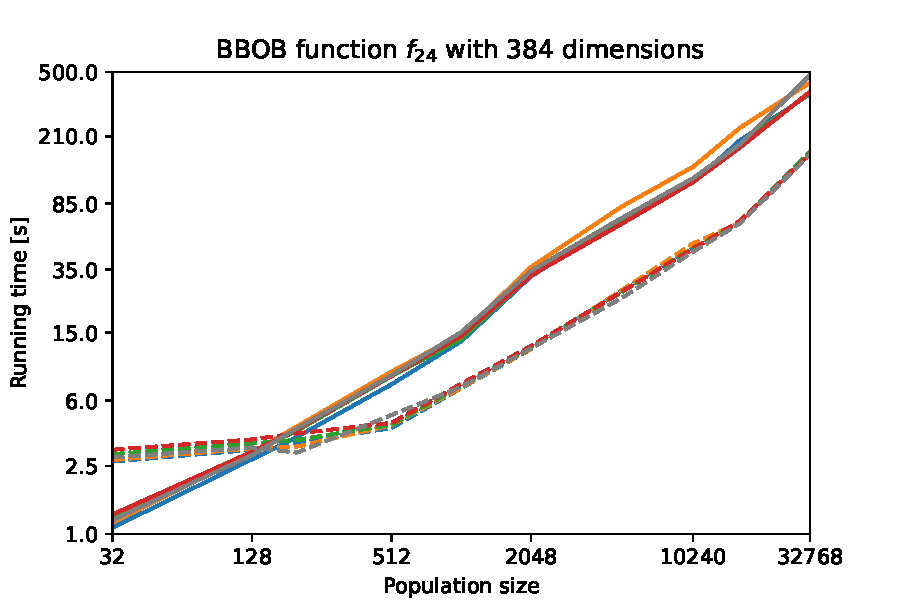
\includegraphics[width=\textwidth]{img/runs/time_es_crossover_fn24_384d.pdf}
    \end{minipage}

    \begin{minipage}{\textwidth}
        \centering
        
\includegraphics[width=\textwidth]{img/runs/time_es_crossover_legend.pdf}
    \end{minipage}

    \caption[Running times of crossover operators]{\todo{Crossover operators running time. Dopsat zbytek.}}
\end{figure}


\begin{figure}[ht!]
    \begin{minipage}[t]{0.32\textwidth}
        \centering
        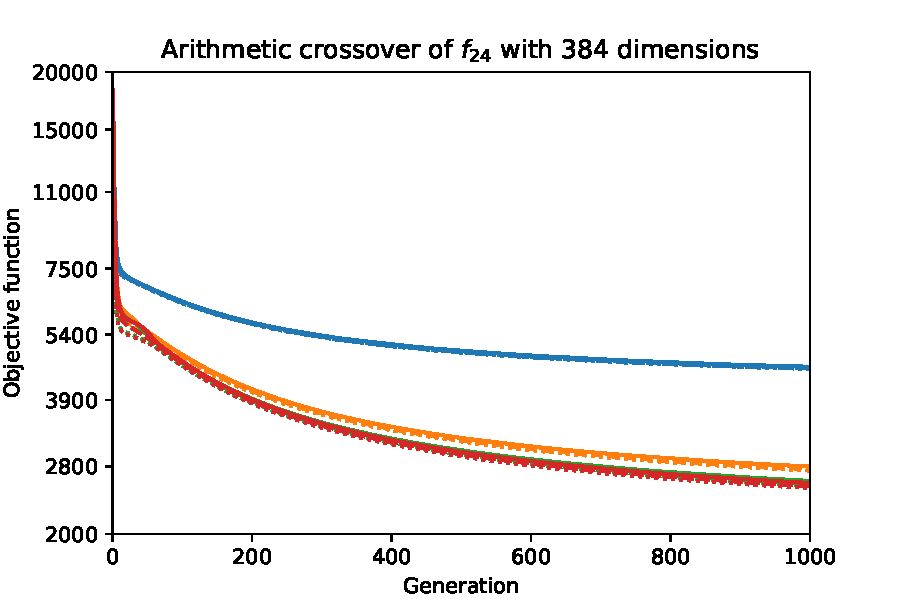
\includegraphics[width=\textwidth]{img/runs/fitness_es_crossover_f24_dim384_Arithmetic.pdf}
    \end{minipage}
    \hfill
    \begin{minipage}[t]{0.32\textwidth}
        \centering
        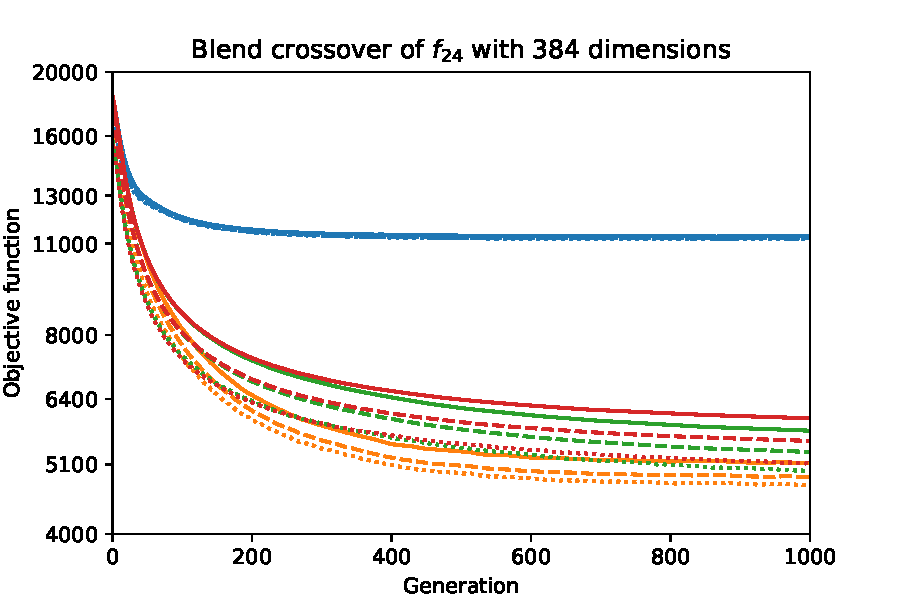
\includegraphics[width=\textwidth]{img/runs/fitness_es_crossover_f24_dim384_Blend.pdf}
    \end{minipage}
    \hfill
    \begin{minipage}[t]{0.32\textwidth}
        \centering
        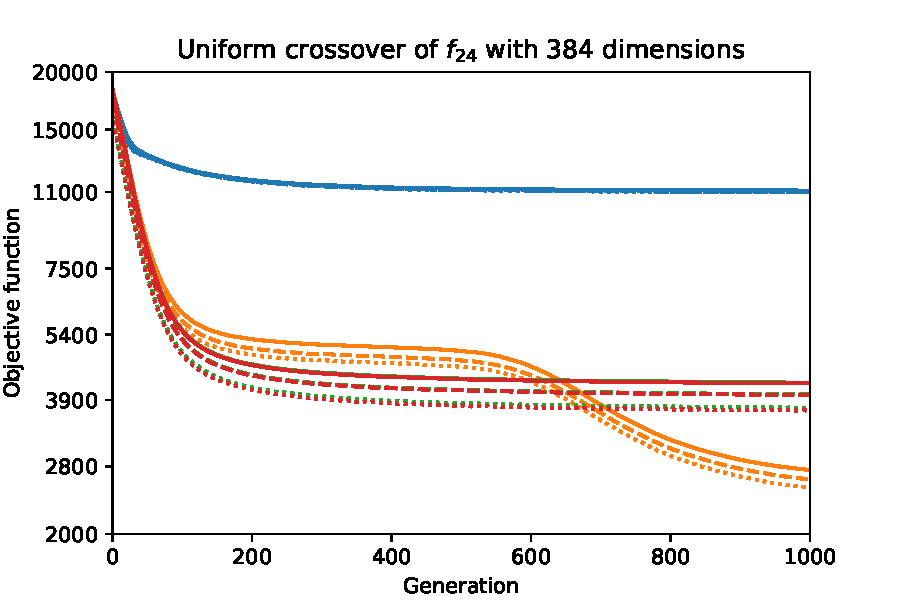
\includegraphics[width=\textwidth]{img/runs/fitness_es_crossover_f24_dim384_Uniform.pdf}
    \end{minipage}
    \\
    \centering
    \begin{minipage}[t]{0.32\textwidth}
        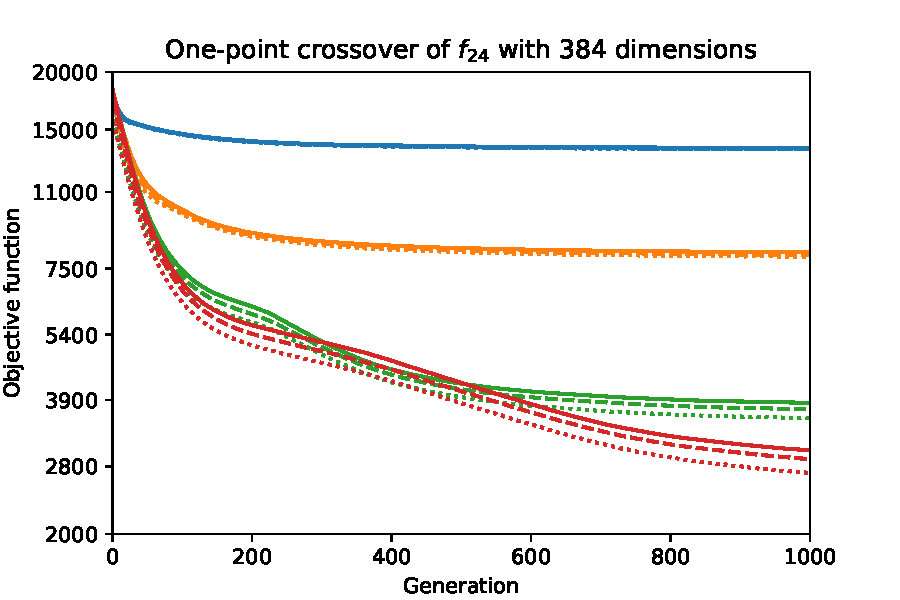
\includegraphics[width=\textwidth]{img/runs/fitness_es_crossover_f24_dim384_OnePoint1D.pdf}
    \end{minipage}
    \begin{minipage}[t]{0.32\textwidth}
        \centering
        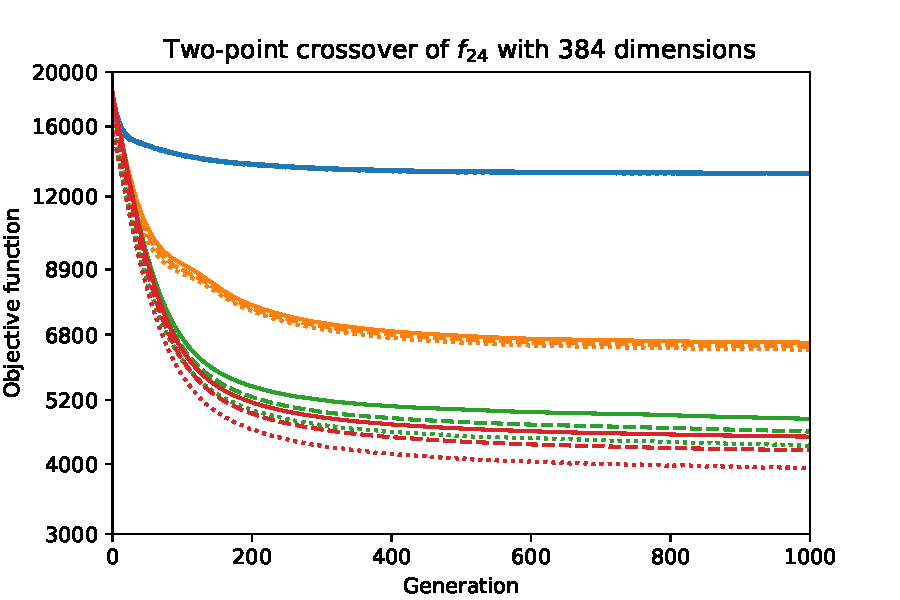
\includegraphics[width=\textwidth]{img/runs/fitness_es_crossover_f24_dim384_TwoPoint1D.pdf}
    \end{minipage}

    \begin{minipage}[t]{0.32\textwidth}
        \centering
        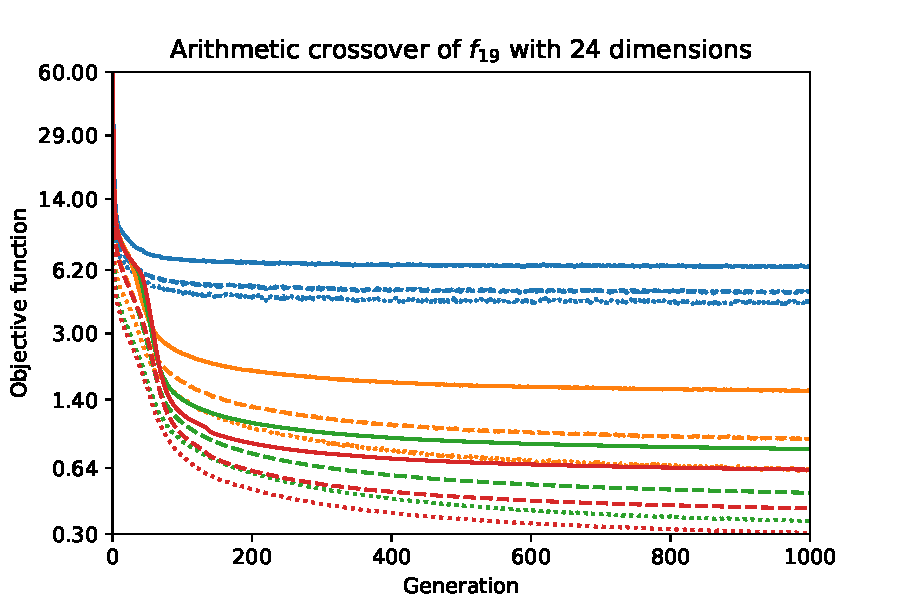
\includegraphics[width=\textwidth]{img/runs/fitness_es_crossover_f19_dim24_Arithmetic.pdf}
    \end{minipage}
    \hfill
    \begin{minipage}[t]{0.32\textwidth}
        \centering
        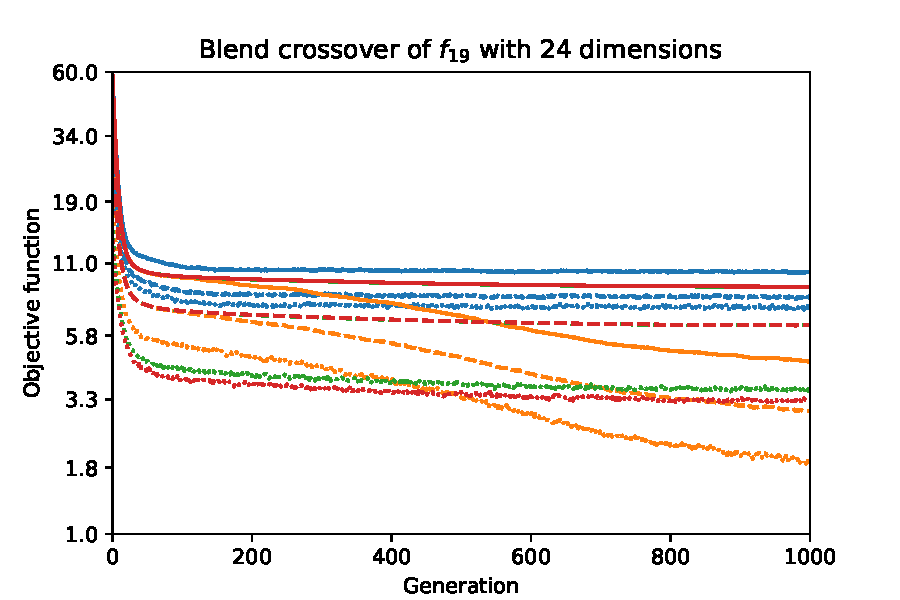
\includegraphics[width=\textwidth]{img/runs/fitness_es_crossover_f19_dim24_Blend.pdf}
    \end{minipage}
    \hfill
    \begin{minipage}[t]{0.32\textwidth}
        \centering
        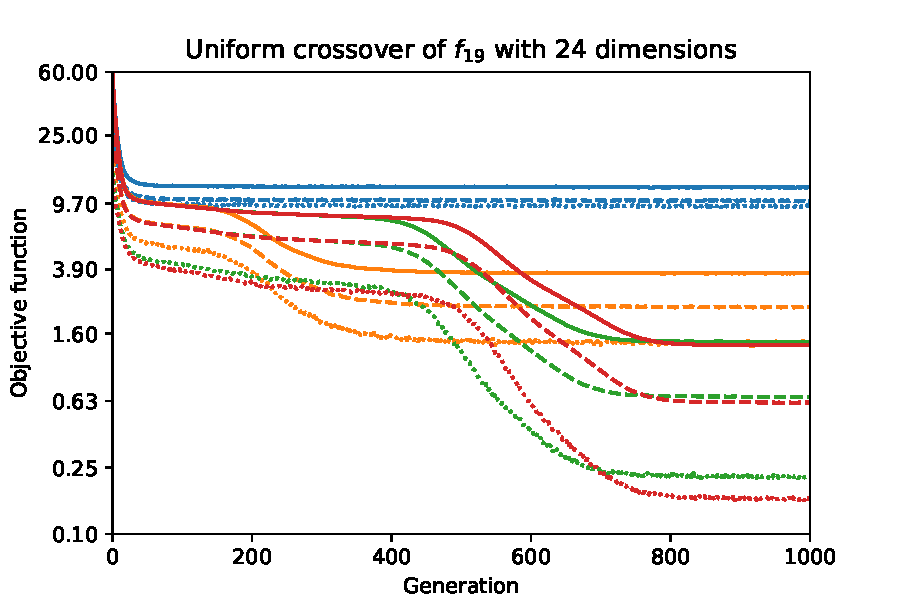
\includegraphics[width=\textwidth]{img/runs/fitness_es_crossover_f19_dim24_Uniform.pdf}
    \end{minipage}
    \\
    \centering
    \begin{minipage}[t]{0.32\textwidth}
        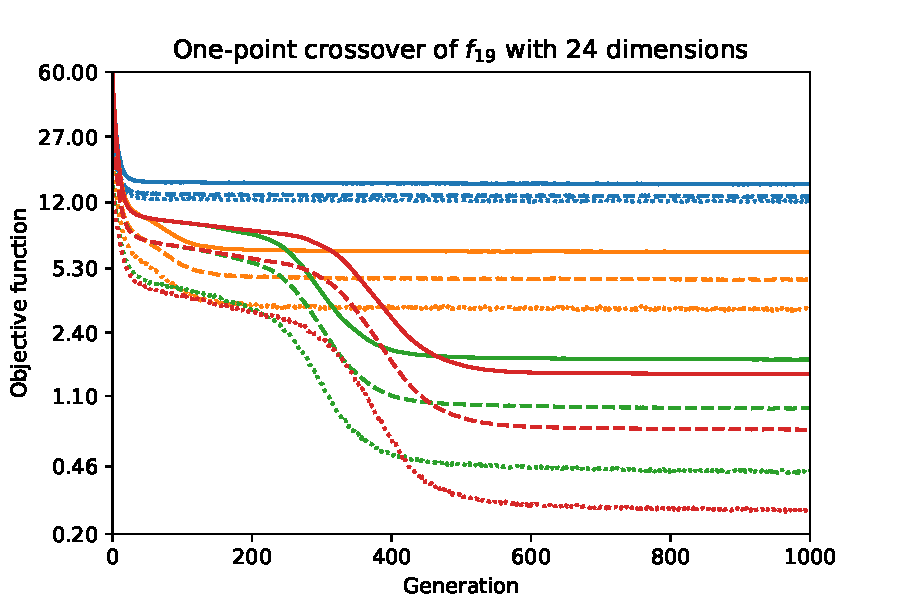
\includegraphics[width=\textwidth]{img/runs/fitness_es_crossover_f19_dim24_OnePoint1D.pdf}
    \end{minipage}
    \begin{minipage}[t]{0.32\textwidth}
        \centering
        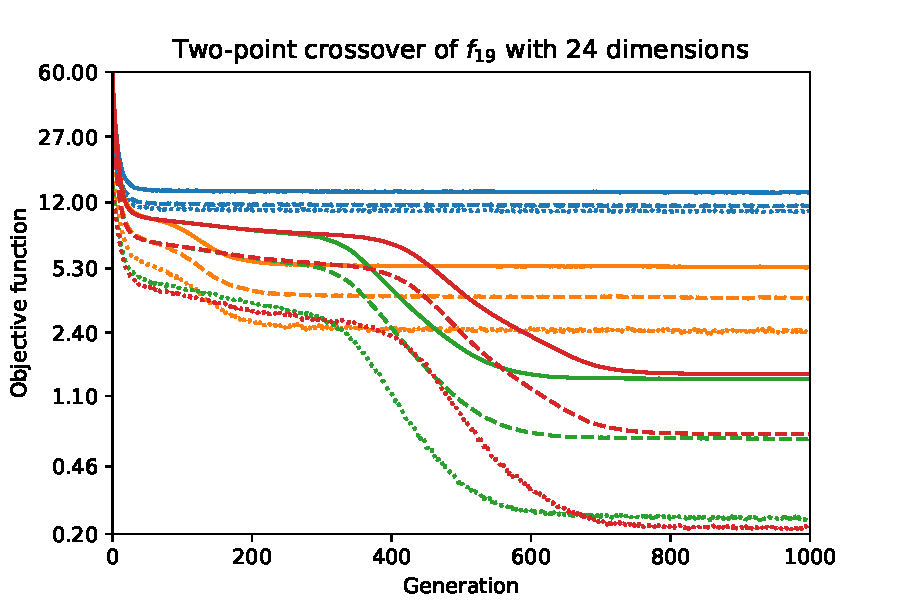
\includegraphics[width=\textwidth]{img/runs/fitness_es_crossover_f19_dim24_TwoPoint1D.pdf}
    \end{minipage}

    \begin{minipage}{\textwidth}
        \centering
        \includegraphics[width=\textwidth]{img/runs/fitness_es_crossovers_legend.pdf}
    \end{minipage}

    \caption[Fitness of crossover operators]{\todo{Fitness of crossover operators. Dopsat zbytek.}}
\end{figure}




%%%%%%%%%%%%%%%%%%%
%%               %%
%%   ES SCHEMA   %%
%%               %%
%5%%%%%%%%%%%%%%%%%
\begin{figure}[ht!]
    \begin{minipage}[t]{0.32\textwidth}
        \centering
        \includegraphics[width=\textwidth]{img/runs/time_es_schema_fn19_24d.pdf}
    \end{minipage}
    \hfill
    \begin{minipage}[t]{0.32\textwidth}
        \centering
        \includegraphics[width=\textwidth]{img/runs/time_es_schema_fn19_128d.pdf}
    \end{minipage}
    \hfill
    \begin{minipage}[t]{0.32\textwidth}
        \centering
        \includegraphics[width=\textwidth]{img/runs/time_es_schema_fn19_384d.pdf}
    \end{minipage}

    \begin{minipage}[t]{0.32\textwidth}
        \centering
        \includegraphics[width=\textwidth]{img/runs/time_es_schema_fn22_24d.pdf}
    \end{minipage}
    \hfill
    \begin{minipage}[t]{0.32\textwidth}
        \centering
        \includegraphics[width=\textwidth]{img/runs/time_es_schema_fn22_128d.pdf}
    \end{minipage}
    \hfill
    \begin{minipage}[t]{0.32\textwidth}
        \centering
        \includegraphics[width=\textwidth]{img/runs/time_es_schema_fn22_384d.pdf}
    \end{minipage}

    \begin{minipage}{\textwidth}
        \centering
        \includegraphics[width=0.8\textwidth]{img/runs/time_es_schema_legend.pdf}
    \end{minipage}

    \caption[Running times crossover schemas]{\todo{Crossover schemas running times. Dopsat zbytek.}}
\end{figure}




%%%%%%%%%%%%%%%%%
%%             %%
%%   PSO2006   %%
%%             %%
%%%%%%%%%%%%%%%%%
\begin{figure}[ht!]
    \begin{minipage}[t]{0.32\textwidth}
        \centering
        \includegraphics[width=\textwidth]{img/runs/time_pso2006_fn1_alldim.pdf}
    \end{minipage}
    \hfill
    \begin{minipage}[t]{0.32\textwidth}
        \centering
        \includegraphics[width=\textwidth]{img/runs/time_pso2006_fn7_alldim.pdf}
    \end{minipage}
    \hfill
    \begin{minipage}[t]{0.32\textwidth}
        \centering
        \includegraphics[width=\textwidth]{img/runs/time_pso2006_fn15_alldim.pdf}
    \end{minipage}

    \begin{minipage}[t]{0.32\textwidth}
        \centering
        \includegraphics[width=\textwidth]{img/runs/time_pso2006_fn19_alldim.pdf}
    \end{minipage}
    \hfill
    \begin{minipage}[t]{0.32\textwidth}
        \centering
        \includegraphics[width=\textwidth]{img/runs/time_pso2006_fn22_alldim.pdf}
    \end{minipage}
    \hfill
    \begin{minipage}[t]{0.32\textwidth}
        \centering
        \includegraphics[width=\textwidth]{img/runs/time_pso2006_fn24_alldim.pdf}
    \end{minipage}

    \begin{minipage}{\textwidth}
        \centering
        \includegraphics[width=\textwidth]{img/runs/time_pso2006_alldim_legend.pdf}
    \end{minipage}

    \caption[PSO2006 running times]{Running times of \acrlong{acc:spso2006} algorithm using problems of dimension $6$, $32$, $128$, and $384$. The algorithm run for $1000$ generations. Populations with over $1000$ particles takes advantage of \gpu and are clearly faster to evaluate.}
\end{figure}

\begin{figure}[ht!]
    \begin{minipage}[t]{0.32\textwidth}
        \centering
        \includegraphics[width=\textwidth]{img/runs/fitness_pso2006_f1.pdf}
    \end{minipage}
    \hfill
    \begin{minipage}[t]{0.32\textwidth}
        \centering
        \includegraphics[width=\textwidth]{img/runs/fitness_pso2006_f7.pdf}
    \end{minipage}
    \hfill
    \begin{minipage}[t]{0.32\textwidth}
        \centering
        \includegraphics[width=\textwidth]{img/runs/fitness_pso2006_f15.pdf}
    \end{minipage}

    \begin{minipage}[t]{0.32\textwidth}
        \centering
        \includegraphics[width=\textwidth]{img/runs/fitness_pso2006_f19.pdf}
    \end{minipage}
    \hfill
    \begin{minipage}[t]{0.32\textwidth}
        \centering
        \includegraphics[width=\textwidth]{img/runs/fitness_pso2006_f22.pdf}
    \end{minipage}
    \hfill
    \begin{minipage}[t]{0.32\textwidth}
        \centering
        \includegraphics[width=\textwidth]{img/runs/fitness_pso2006_f24.pdf}
    \end{minipage}

    \begin{minipage}{\textwidth}
        \centering
        \includegraphics[width=\textwidth]{img/runs/fitness_pso2011_legend.pdf}
    \end{minipage}

    \caption[PSO2006 fitness over generations]{Median, $0.05$ quantile, and best fitness of \acrlong{acc:spso2006} algorithm using random neighborhood on problem with $128$ dimensions. I measured populations consisting of $32$, $512$, $10240$, and $32768$ particles. All the problem functions take advantage of more particles, except of function $f_7$. Given hyperparameters in table \ref{tab:psohyperparameters}, \acrshort{acc:spso2006} seems to have better convergence properties in comparison to \acrshort{acc:spso2011}.}
\end{figure}




%%%%%%%%%%%%%%%%%%%%%%%%%%
%%                      %%
%%   PSO NEIGHBORHOOD   %%
%%                      %%
%%%%%%%%%%%%%%%%%%%%%%%%%%
\begin{figure}[ht!]
    \begin{minipage}[t]{0.32\textwidth}
        \centering
        \includegraphics[width=\textwidth]{img/runs/time_pso2006_fn1_neigh.pdf}
    \end{minipage}
    \hfill
    \begin{minipage}[t]{0.32\textwidth}
        \centering
        \includegraphics[width=\textwidth]{img/runs/time_pso2006_fn7_neigh.pdf}
    \end{minipage}
    \hfill
    \begin{minipage}[t]{0.32\textwidth}
        \centering
        \includegraphics[width=\textwidth]{img/runs/time_pso2006_fn15_neigh.pdf}
    \end{minipage}

    \begin{minipage}[t]{0.32\textwidth}
        \centering
        \includegraphics[width=\textwidth]{img/runs/time_pso2006_fn19_neigh.pdf}
    \end{minipage}
    \hfill
    \begin{minipage}[t]{0.32\textwidth}
        \centering
        \includegraphics[width=\textwidth]{img/runs/time_pso2006_fn22_neigh.pdf}
    \end{minipage}
    \hfill
    \begin{minipage}[t]{0.32\textwidth}
        \centering
        \includegraphics[width=\textwidth]{img/runs/time_pso2006_fn24_neigh.pdf}
    \end{minipage}

    \begin{minipage}{\textwidth}
        \centering
        \includegraphics[width=0.5\textwidth]{img/runs/time_pso_neigh_legend.pdf}
    \end{minipage}

    \caption[PSO2006 neighborhood running times]{Running times of \acrlong{acc:spso2011} algorithm with different neighborhood types. The algorithm run for 1000 generations on problem with 128 dimensions. Neighborhood sizes are at table \ref{tab:psohyperparameters}. The nearest neighborhood topology was run only to population of size 4900, as it compares all pairs of individuals and the device does not have enough memory. The minimum population size for grid topologies were 225, because topologies size were specified as a fraction of population size and for smaller populations neighborhood could not be constructed. The grid topologies were always assembled into square. Running times of circle, linear grid, compact grid, and diamond grid were almost identical (depending only on the size of neighborhood, see chapter \ref{chap:impl}), so I plot only measurements for circle and diamond grid.}
\end{figure}



\begin{figure}[ht!]
    \begin{minipage}[t]{0.32\textwidth}
        \centering
        \includegraphics[width=\textwidth]{img/runs/fitness_pso_f24_neighRandom.pdf}
    \end{minipage}
    \hfill
    \begin{minipage}[t]{0.32\textwidth}
        \centering
        \includegraphics[width=\textwidth]{img/runs/fitness_pso_f24_neighNearest.pdf}
    \end{minipage}
    \hfill
    \begin{minipage}[t]{0.32\textwidth}
        \centering
        \includegraphics[width=\textwidth]{img/runs/fitness_pso_f24_neighCircle.pdf}
    \end{minipage}

    \begin{minipage}[t]{0.32\textwidth}
        \centering
        \includegraphics[width=\textwidth]{img/runs/fitness_pso_f24_neighLinearGrid.pdf}
    \end{minipage}
    \hfill
    \begin{minipage}[t]{0.32\textwidth}
        \centering
        \includegraphics[width=\textwidth]{img/runs/fitness_pso_f24_neighCompactGrid.pdf}
    \end{minipage}
    \hfill
    \begin{minipage}[t]{0.32\textwidth}
        \centering
        \includegraphics[width=\textwidth]{img/runs/fitness_pso_f24_neighDiamondGrid.pdf}
    \end{minipage}

    \begin{minipage}{\textwidth}
        \centering
        \includegraphics[width=0.8\textwidth]{img/runs/fitness_pso_neigh_legend.pdf}
    \end{minipage}

    \caption[PSO neighborhood fitness]{Fitness of neighborhoods using $121$, $529$, $4900$, and $22500$ particles and \acrshort{acc:spso2006} update algorithm. Nearest neighborhood for $22500$ particles is not present, because of the memory demands. Grid neighborhoods for $121$ particles is not present, because there was not enough particles to build it. 
    All the neighborhoods clearly benefit from greater number of particles with the exception of compact grid and diamond grid. This is probably caused by premature convergence rather than degredation of the performance.
    Measurements for \acrshort{acc:bbob} functions $f_1$, $f_7$, $f_{15}$, and $f_{22}$ report similar properties.}
\end{figure}




%%%%%%%%%%%%%%%%%
%%             %%
%%   PSO2011   %%
%%             %%
%%%%%%%%%%%%%%%%%
\begin{figure}[ht!]
    \begin{minipage}[t]{0.32\textwidth}
        \centering
        \includegraphics[width=\textwidth]{img/runs/time_pso2011_fn1_alldim.pdf}
    \end{minipage}
    \hfill
    \begin{minipage}[t]{0.32\textwidth}
        \centering
        \includegraphics[width=\textwidth]{img/runs/time_pso2011_fn7_alldim.pdf}
    \end{minipage}
    \hfill
    \begin{minipage}[t]{0.32\textwidth}
        \centering
        \includegraphics[width=\textwidth]{img/runs/time_pso2011_fn15_alldim.pdf}
    \end{minipage}

    \begin{minipage}[t]{0.32\textwidth}
        \centering
        \includegraphics[width=\textwidth]{img/runs/time_pso2011_fn19_alldim.pdf}
    \end{minipage}
    \hfill
    \begin{minipage}[t]{0.32\textwidth}
        \centering
        \includegraphics[width=\textwidth]{img/runs/time_pso2011_fn22_alldim.pdf}
    \end{minipage}
    \hfill
    \begin{minipage}[t]{0.32\textwidth}
        \centering
        \includegraphics[width=\textwidth]{img/runs/time_pso2011_fn24_alldim.pdf}
    \end{minipage}

    \begin{minipage}{\textwidth}
        \centering
        \includegraphics[width=\textwidth]{img/runs/time_pso2011_alldim_legend.pdf}
    \end{minipage}

    \caption[PSO2011 running times]{Running times of \acrlong{acc:spso2011} algorithm using problems of dimension $6$, $32$, $128$, and $384$. The algorithm run for $1000$ generations. Populations with over $1000$ particles takes clear advantage of \gpu.}
\end{figure}

\begin{figure}[ht!]
    \begin{minipage}[t]{0.32\textwidth}
        \centering
        \includegraphics[width=\textwidth]{img/runs/fitness_pso2011_f1.pdf}
    \end{minipage}
    \hfill
    \begin{minipage}[t]{0.32\textwidth}
        \centering
        \includegraphics[width=\textwidth]{img/runs/fitness_pso2011_f7.pdf}
    \end{minipage}
    \hfill
    \begin{minipage}[t]{0.32\textwidth}
        \centering
        \includegraphics[width=\textwidth]{img/runs/fitness_pso2011_f15.pdf}
    \end{minipage}

    \begin{minipage}[t]{0.32\textwidth}
        \centering
        \includegraphics[width=\textwidth]{img/runs/fitness_pso2011_f19.pdf}
    \end{minipage}
    \hfill
    \begin{minipage}[t]{0.32\textwidth}
        \centering
        \includegraphics[width=\textwidth]{img/runs/fitness_pso2011_f22.pdf}
    \end{minipage}
    \hfill
    \begin{minipage}[t]{0.32\textwidth}
        \centering
        \includegraphics[width=\textwidth]{img/runs/fitness_pso2011_f24.pdf}
    \end{minipage}

    \begin{minipage}{\textwidth}
        \centering
        \includegraphics[width=\textwidth]{img/runs/fitness_pso2011_legend.pdf}
    \end{minipage}

    \caption[PSO2011 fitness over generations]{Median, $0.05$ quantile, and best fitness of \acrlong{acc:spso2011} algorithm using random neighborhood on problem with $128$ dimensions. I measured populations consisting of $32$, $512$, $10240$, and $32768$ particles. All the problem functions take advantage of more particles.}
\end{figure}

\chapter{Digital attachments}

Digital version of this work with all the attachments is also available at my GitHub repository at \url{https://github.com/PatrikValkovic/MasterThesis}.

\begin{figure}
    \dirtree{%
        .1 thesis\DTcomment{thesis in the \LaTeX format}.
            .2 img\DTcomment{figures used in this thesis}.
        .1 src\DTcomment{source codes used for this work}.
            .2 BBOBtorch\DTcomment{implementation of \acrshort{acc:bbob} functions in PyTorch}.
            .2 FFEAT\DTcomment{implementation of \acrshort{acc:ffeat} library}.
            .2 Scripts\DTcomment{Script used for evaluation and measurement}.
        .1 thesis.pdf\DTcomment{thesis in the digital version}.
    }
\end{figure}

\openright
\end{document}
